% Options for packages loaded elsewhere
\PassOptionsToPackage{unicode}{hyperref}
\PassOptionsToPackage{hyphens}{url}
\documentclass[
  11pt,
]{article}
\usepackage{xcolor}
\usepackage[margin=22mm]{geometry}
\usepackage{amsmath,amssymb}
\setcounter{secnumdepth}{-\maxdimen} % remove section numbering
\usepackage{iftex}
\ifPDFTeX
  \usepackage[T1]{fontenc}
  \usepackage[utf8]{inputenc}
  \usepackage{textcomp} % provide euro and other symbols
\else % if luatex or xetex
  \usepackage{unicode-math} % this also loads fontspec
  \defaultfontfeatures{Scale=MatchLowercase}
  \defaultfontfeatures[\rmfamily]{Ligatures=TeX,Scale=1}
\fi
\usepackage{lmodern}
\ifPDFTeX\else
  % xetex/luatex font selection
\fi
% Use upquote if available, for straight quotes in verbatim environments
\IfFileExists{upquote.sty}{\usepackage{upquote}}{}
\IfFileExists{microtype.sty}{% use microtype if available
  \usepackage[]{microtype}
  \UseMicrotypeSet[protrusion]{basicmath} % disable protrusion for tt fonts
}{}
\makeatletter
\@ifundefined{KOMAClassName}{% if non-KOMA class
  \IfFileExists{parskip.sty}{%
    \usepackage{parskip}
  }{% else
    \setlength{\parindent}{0pt}
    \setlength{\parskip}{6pt plus 2pt minus 1pt}}
}{% if KOMA class
  \KOMAoptions{parskip=half}}
\makeatother
\usepackage{graphicx}
\makeatletter
\newsavebox\pandoc@box
\newcommand*\pandocbounded[1]{% scales image to fit in text height/width
  \sbox\pandoc@box{#1}%
  \Gscale@div\@tempa{\textheight}{\dimexpr\ht\pandoc@box+\dp\pandoc@box\relax}%
  \Gscale@div\@tempb{\linewidth}{\wd\pandoc@box}%
  \ifdim\@tempb\p@<\@tempa\p@\let\@tempa\@tempb\fi% select the smaller of both
  \ifdim\@tempa\p@<\p@\scalebox{\@tempa}{\usebox\pandoc@box}%
  \else\usebox{\pandoc@box}%
  \fi%
}
% Set default figure placement to htbp
\def\fps@figure{htbp}
\makeatother
\usepackage{svg}
\setlength{\emergencystretch}{3em} % prevent overfull lines
\providecommand{\tightlist}{%
  \setlength{\itemsep}{0pt}\setlength{\parskip}{0pt}}
\usepackage{bookmark}
\IfFileExists{xurl.sty}{\usepackage{xurl}}{} % add URL line breaks if available
\urlstyle{same}
\hypersetup{
  hidelinks,
  pdfcreator={LaTeX via pandoc}}

\author{}
\date{}

\ExplSyntaxOn
\cs_new:Npn \ReaderIfNativeAnchorTF #1 { \exp_args:Nx \str_if_in:nnTF {#1} {section*.} }
\ExplSyntaxOff
\makeatletter
\let\ReaderOriginalAnchorStart\hyper@anchorstart
\let\ReaderOriginalAnchorEnd\hyper@anchorend
\let\ReaderPendingAliases\@empty
\def\ReaderArmAliases#1{\gdef\ReaderPendingAliases{#1}}
\def\hyper@anchorstart#1{\ReaderIfNativeAnchorTF{#1}{\ReaderPendingAliases\global\let\ReaderPendingAliases\@empty}{}\ReaderOriginalAnchorStart{#1}}
\makeatother
\begin{document}

\ReaderArmAliases{\ReaderOriginalAnchorStart{when-a-nonnegative-scalar-symbol-acquires-a-negative-part}\ReaderOriginalAnchorEnd}
\section{When a nonnegative scalar symbol acquires a negative
part}\label{when-a-nonnegative-scalar-symbol-acquires-a-negative-part}

A nonnegative function on phase space need not quantize to a nonnegative
operator. Nevertheless its negative quadratic form can be bounded by a
constant when the symbol has the appropriate size relative to its
derivative scale. For scalar symbols the permitted size is the inverse
square of the local Planck parameter. The extra power comes from a
decomposition of a nonnegative function into a square and a function
missing one phase direction. This is a scalar argument; it is not a
theorem about positive matrices or arbitrary Hilbert space operators.

We will build the estimate around two operations that preserve lower
bounds: taking an operator square and integrating a lower-dimensional
estimate with a parameter. A separate localization lemma accounts for
the errors when these local constructions are assembled. The small-scale
construction and the subsequent passage to an arbitrary metric are
different steps of the proof.

Use the Fourier convention \(D=-i\partial\), Lebesgue measure on
\(\mathbb R^n\), and \[
a^wu(x)=(2\pi)^{-n}\iint e^{i(x-y)\cdot\xi}
 a((x+y)/2,\xi)u(y)\,dy\,d\xi.
\tag{F1}
\] The integral is interpreted by the Schwartz-distribution construction
of Section 4 of \href{weyl-metric-products.pdf}{Two measuring scales, one
Weyl product} and Section 4 of \href{weyl-covariance-action.pdf}{From
Weyl symbols to operators and changes of coordinates}. All operator
inequalities below are quadratic-form inequalities on
\(\mathcal S(\mathbb R^n)\). They do not assert that an unbounded
operator has already been given a self-adjoint realization.

The proof uses four kinds of prerequisites.

\begin{itemize}
\tightlist
\item
  \textbf{Metric constructions.} Sections 1--4 of
  \href{metric-localization.pdf}{Localizing symbols with moving metrics}
  give the symbol seminorms, slowly varying ellipsoid covers, uniformly
  differentiable cutoffs, and reconstruction. Sections 1--3 of
  \href{weyl-metric-products.pdf}{Two measuring scales, one Weyl product}
  give symplectic duality, temperate weights, and the Planck parameter.
  Section 5 of \href{weyl-covariance-action.pdf}{From Weyl symbols to
  operators and changes of coordinates} gives the conformal enlargement
  theorem, including nonsmooth metrics.
\item
  \textbf{Weyl calculus.} Section 7 of
  \href{weyl-metric-products.pdf}{Two measuring scales, one Weyl product}
  gives the Weyl product and every finite remainder for compatible
  temperate metrics. For one metric the remainder after terms of order
  less than \(N\) has weight \(m_1m_2h^N\). Section 4 of
  \href{weyl-covariance-action.pdf}{From Weyl symbols to operators and
  changes of coordinates} and Section 6 of
  \href{weyl-covariance-action.pdf}{From Weyl symbols to operators and
  changes of coordinates} give Schwartz action and unitary affine
  symplectic covariance. Section 7 of
  \href{weyl-covariance-action.pdf}{From Weyl symbols to operators and
  changes of coordinates} gives change of quantization with its finite
  remainders.
\item
  \textbf{Operator bounds.} The general-metric continuity theorem in
  Section 7 of \href{metric-operator-bounds.pdf}{When a moving symbol
  scale controls an operator} supplies the following precise interface:
  for a slowly varying symplectically temperate metric
  \(g\leq g^\sigma\), a symbol in \(S(1,g;\mathcal L(H_1,H_2))\) defines
  a bounded operator on \(L^2\), with a norm controlled by finitely many
  symbol seminorms and the metric's structural constants. Constants are
  independent of the Hilbert spaces and of pointwise eccentricity.
  Section 1 of \href{metric-operator-bounds.pdf}{When a moving symbol
  scale controls an operator} supplies the operator-norm version of the
  preceding Weyl product and every finite remainder estimate, preserving
  multiplication order and matching intermediate coefficient spaces.
  Constant metrics have uniform structural constants. The boundedness
  result used here supplies no positivity theorem.
\item
  \textbf{Elementary analytic tools.}
  \href{metric-foundation-bridges.pdf}{The metric and
  calculus lesson, Sections12--14}, proves compactness and extrema,
  complete Taylor/product/chain formulas and smooth cutoffs.
  \href{prerequisite-bridges.pdf}{The Fourier lesson,
  Sections1--3 and7--8}, proves scalar Fourier inversion, Plancherel,
  distribution duality and both real self-adjoint and skew-adjoint
  spectral decompositions with the original inner product.
  \href{geometric-microlocal-calculus.pdf}{The
  geometric lesson, Sections16.4--16.5}, proves the full inverse and
  implicit maps.
  \href{banach-foundation-bridges.pdf}{The Banach
  and measure lesson, Sections16--17}, proves product integration,
  dominated convergence and integration of Hilbert-valued functions
  without an ambient separability assumption. These are the exact
  independent providers; the splitting and induction arguments for
  positivity follow below.
\end{itemize}

\ReaderArmAliases{\ReaderOriginalAnchorStart{AN03-SFP-001}\ReaderOriginalAnchorEnd\begingroup\expandafter\def\csname @currentHref\endcsname{AN03-SFP-001}\label{AN03-SFP-001}\endgroup\ReaderOriginalAnchorStart{an03-sfp-001-the-scale-in-the-two-lower-bounds}\ReaderOriginalAnchorEnd\begingroup\expandafter\def\csname @currentHref\endcsname{an03-sfp-001-the-scale-in-the-two-lower-bounds}\label{an03-sfp-001-the-scale-in-the-two-lower-bounds}\endgroup\ReaderOriginalAnchorStart{1-the-scale-in-the-two-lower-bounds}\ReaderOriginalAnchorEnd\begingroup\expandafter\def\csname @currentHref\endcsname{1-the-scale-in-the-two-lower-bounds}\label{1-the-scale-in-the-two-lower-bounds}\endgroup\ReaderOriginalAnchorStart{the-scale-in-the-two-lower-bounds}\ReaderOriginalAnchorEnd}
\subsection{1. The scale in the two lower
bounds}\label{the-scale-in-the-two-lower-bounds}

On \(E=\mathbb R_x^n\times\mathbb R_\xi^n\) use
\(\sigma((x,\xi),(y,\eta))=\xi\cdot y-x\cdot\eta\). For a positive
quadratic form \(g_X\), put \[
g_X^\sigma(T)=\sup_{S\ne0}\frac{|\sigma(T,S)|^2}{g_X(S)},
\qquad h(X)^2=\sup_{T\ne0}\frac{g_X(T)}{g_X^\sigma(T)}.
\tag{F2}
\] Here a permissible metric means a slowly varying, symplectically
temperate metric satisfying \(h\leq1\). Symplectic temperateness has the
distance base specified in Section 2 of
\href{weyl-metric-products.pdf}{Two measuring scales, one Weyl product};
for example it can be written \[
g_Y\leq Cg_X\bigl(1+g_Y^\sigma(X-Y)\bigr)^N.
\tag{F3}
\] No ordinary smoothness of \(X\mapsto g_X\) is assumed. The seminorms
are the multilinear derivative seminorms of Section 1 of
\href{metric-localization.pdf}{Localizing symbols with moving metrics}.
In particular \(a\in S(h^{-j},g)\) means \[
|a^{(k)}(X)[T_1,\ldots,T_k]|
 \leq C_k h(X)^{-j}\prod_{l=1}^k g_X(T_l)^{1/2}.
\tag{F4}
\] The Planck parameter and its powers are temperate weights. To verify
the point needed here, compare \(g_X\) with \(g_Y\) in (F3), dualize
that comparison, and take the supremum defining (F2). The resulting
ratio of Planck parameters is bounded by a power of the same distance.
Local comparisons follow by the same argument from slow variation.

Both estimates here concern scalar symbols. Our two conclusions are \[
\begin{array}{ll}
0\leq a\in S(h^{-1},g)&\Longrightarrow\quad
 \langle a^wu,u\rangle\geq-C\|u\|^2,\\
0\leq a\in S(h^{-2},g),\quad a\text{ scalar}
 &\Longrightarrow\quad\langle a^wu,u\rangle\geq-C\|u\|^2.
\end{array}
\tag{F5}
\] The first will follow from one adapted square root. The second, the
scalar Fefferman--Phong estimate, will follow from dimension induction.
Constants depend on finitely many seminorms of \(a\), the dimension and
the structural constants of \(g\). They are uniform on sets on which
these data are bounded. The proof will explain why finitely many
derivatives suffice; no optimal derivative count is claimed.

\ReaderArmAliases{\ReaderOriginalAnchorStart{AN03-SFP-002}\ReaderOriginalAnchorEnd\begingroup\expandafter\def\csname @currentHref\endcsname{AN03-SFP-002}\label{AN03-SFP-002}\endgroup\ReaderOriginalAnchorStart{an03-sfp-002-a-square-root-measured-at-its-own-scale}\ReaderOriginalAnchorEnd\begingroup\expandafter\def\csname @currentHref\endcsname{an03-sfp-002-a-square-root-measured-at-its-own-scale}\label{an03-sfp-002-a-square-root-measured-at-its-own-scale}\endgroup\ReaderOriginalAnchorStart{2-a-square-root-measured-at-its-own-scale}\ReaderOriginalAnchorEnd\begingroup\expandafter\def\csname @currentHref\endcsname{2-a-square-root-measured-at-its-own-scale}\label{2-a-square-root-measured-at-its-own-scale}\endgroup\ReaderOriginalAnchorStart{a-square-root-measured-at-its-own-scale}\ReaderOriginalAnchorEnd}
\subsection{2. A square root measured at its own
scale}\label{a-square-root-measured-at-its-own-scale}

We first prove the first line of (F5). A basic positivity estimate will
be useful. If \(F\geq0\) on a fixed ball, \(F\) and its second
derivatives are bounded there, then on a smaller concentric ball \[
|F'(z)|\leq C F(z)^{1/2}.
\tag{F6}
\] For a unit direction \(v\), Taylor's formula gives
\(0\leq F(z+tv)\leq F(z)+tF'(z)v+Ct^2\) in both signs of \(t\). Choosing
the sign opposite to \(F'(z)v\) gives \(|F'(z)v|\leq F(z)/s+Cs\) for
every allowed \(s>0\). If \(F(z)\) is small choose \(s\) proportional to
\(F(z)^{1/2}\); otherwise use a fixed \(s\) and the boundedness of
\(F\). The case \(F(z)=0\) follows by letting \(s\downarrow0\). Taking
the supremum over directions proves (F6).

Let \(a\geq0\) belong to \(S(h^{-1},g)\), and set \[
m=a+1,\qquad G_X=\frac{g_X}{h(X)m(X)}.
\tag{F7}
\] At a fixed point \(X\), choose \(g_X\)-orthonormal coordinates \(z\)
centered at \(X\). Slow variation of \(g,h\) makes \(F(z)=h(X)a(X+z)\)
and all its derivatives uniformly bounded on a fixed coordinate ball.
Applying (F6) at its center gives \[
|a'(X)T|\leq C\sqrt{a(X)/h(X)}\,g_X(T)^{1/2}.
\tag{F8}
\] For \(k\geq2\), the original symbol estimate implies \[
|a^{(k)}(X)[T_1,\ldots,T_k]|
\leq C_k m(X)^{1-k/2}h(X)^{-k/2}
             \prod_l g_X(T_l)^{1/2}.
\tag{F9}
\] Indeed \(h m\) is bounded above, and division of the right side by
\(h^{-1}\prod g_X(T_l)^{1/2}\) gives \((hm)^{1-k/2}\), bounded below by
a positive constant. For \(k=1\), (F9) follows from (F8). Thus
\(m\in S(m,G)\).

We check the metric assumptions rather than assuming a smooth square
root has already solved the problem. In the coordinates just used, \[
|F(z)-F(0)|\leq C\sqrt{F(0)}|z|+C|z|^2.
\tag{F10}
\] If \(|z|\leq c\sqrt{F(0)+h(X)}\), with \(c\) fixed sufficiently
small, this is at most \((F(0)+h(X))/2\). Such a displacement lies
inside the original coordinate ball since \(hm\) is uniformly bounded.
Consequently \(a(X+z)+1\) and \(a(X)+1\) are comparable, as are \(g,h\).
This is exactly slow variation of \(G\). Quadratic scaling gives \[
h_G=\frac1m\leq1.
\tag{F11}
\] The original conformal multiplier in (F7) satisfies the explicit
bound \[
 \mu(X)=\frac1{h(X)m(X)}\ge\mu_0,
 \qquad \mu_0=\frac1{1+p_0(a;h^{-1},g)}>0,
 \tag{F11a}
\] because \(h(X)a(X)\le p_0(a;h^{-1},g)\) and \(h(X)\le1\). Keep the
original \(g\) and this exact \(G\). Equations (A56)--(A58) of
\href{weyl-covariance-action.pdf}{From Weyl symbols to operators and
changes of coordinates} apply with precisely (F11a), the slow variation
just proved, and (F11). They prove temperateness of \(G\), including the
distance base and dependence on \(\mu_0\). No metric is replaced. This
argument does not require the multiplier or \(h\) to be smooth. Equation
(F11), with the Planck-parameter weight comparison proved after (F4),
also proves temperateness of \(m\) for \(G\).

For completeness, if \(M>0\) is a smooth symbol in \(S(M,G)\) and a
positive smooth scalar function \(F\) satisfies
\(|t^jF^{(j)}(t)|\leq C_jF(t)\), the chain rule indexed by set
partitions gives \[
D^k(F(M))=
 \sum_{\pi}F^{(|\pi|)}(M)
          \prod_{B\in\pi}D^{|B|}M.
\tag{F12}
\] The powers of \(M\) cancel in each term. The bound on the first
logarithmic derivative also gives
\(|\log F(t)-\log F(s)|\leq C|\log(t/s)|\), so local comparison and
temperateness of \(M\) imply the same properties for \(F(M)\). This
proves \(F(M)\in S(F(M),G)\). In particular
\(b=\sqrt m\in S(m^{1/2},G)\). The first Weyl correction of \(b\#b\)
vanishes because the Poisson bracket of a scalar function with itself is
zero. The order-two remainder gives \[
b\#b=m+r,\qquad r\in S(mh_G^2,G)=S(m^{-1},G)\subset S(1,G).
\tag{F13}
\] The operator \(r^w\) is bounded by Section 7 of
\href{metric-operator-bounds.pdf}{When a moving symbol scale controls an
operator}. Since \(b\) is real, \(\langle(b^w)^2u,u\rangle=\|b^wu\|^2\)
on Schwartz functions. Thus
\(\langle a^wu,u\rangle=\|b^wu\|^2-\|u\|^2-\langle r^wu,u\rangle\),
proving the first line of (F5).

\ReaderArmAliases{\ReaderOriginalAnchorStart{AN03-SFP-003}\ReaderOriginalAnchorEnd\begingroup\expandafter\def\csname @currentHref\endcsname{AN03-SFP-003}\label{AN03-SFP-003}\endgroup\ReaderOriginalAnchorStart{an03-sfp-003-what-four-derivatives-and-nonnegativity-control}\ReaderOriginalAnchorEnd\begingroup\expandafter\def\csname @currentHref\endcsname{an03-sfp-003-what-four-derivatives-and-nonnegativity-control}\label{an03-sfp-003-what-four-derivatives-and-nonnegativity-control}\endgroup\ReaderOriginalAnchorStart{3-what-four-derivatives-and-nonnegativity-control}\ReaderOriginalAnchorEnd\begingroup\expandafter\def\csname @currentHref\endcsname{3-what-four-derivatives-and-nonnegativity-control}\label{3-what-four-derivatives-and-nonnegativity-control}\endgroup\ReaderOriginalAnchorStart{what-four-derivatives-and-nonnegativity-control}\ReaderOriginalAnchorEnd}
\subsection{3. What four derivatives and nonnegativity
control}\label{what-four-derivatives-and-nonnegativity-control}

Here \(B_r\subset\mathbb R^d\) is the Euclidean ball of radius \(r\).
For this finite-dimensional lemma only, write
\(j_k(f,x)=\sup_{|v|=1}|D^kf(x)[v,\ldots,v]|\). These diagonal seminorms
are equivalent to multilinear norms by polarization; all constants below
may depend on \(d,k\). For \(k\leq3\), real symmetric derivatives have
exactly the same diagonal and multilinear norms. Thus the numerical
bounds below also hold in the multilinear convention of Section 1 of
\href{metric-localization.pdf}{Localizing symbols with moving metrics}.
The cases \(k\leq1\) are immediate, and \(k=2\) is the spectral norm
identity for a real symmetric matrix.

Here is a finite-dimensional proof for \(k=3\), to retain the numerical
constants. Let \(T\) be a real symmetric trilinear form and \(M\) its
multilinear norm. The zero form is immediate. Among unit triples
attaining \(|T(x,y,z)|=M\), choose one maximizing \(\|x+y+z\|\), using
compactness. Fix \(z\) and let \(B\) be the symmetric operator with
\(\langle Bx,y\rangle=T(x,y,z)\). At an extremal triple, differentiation
on each unit sphere gives \(Bx=\varepsilon My\) and
\(By=\varepsilon Mx\), where \(\varepsilon\) is the sign of
\(T(x,y,z)\). If \(0<r=\|x+y\|<2\), set \(v=(x+y)/r\). Then
\(Bv=\varepsilon Mv\), so \((v,v,z)\) is another maximizing triple. Its
squared sum norm exceeds the previous one by \[
(2-r)\bigl(2+r+2\langle v,z\rangle\bigr)\geq(2-r)r>0,
\] a contradiction. If \(x=-y\), replacing the pair by \((v,v)\), where
\(v\) is either \(x\) or \(-x\) and \(\langle v,z\rangle\geq0\),
preserves the absolute trilinear value and increases the squared sum
norm from one to at least five. Hence \(x=y\). Applying the same
argument to each pair shows \(x=y=z\), which proves equality with the
diagonal norm. At order four we only need that a multilinear bound
implies the same diagonal bound, and that polarization controls mixed
derivatives by a fixed dimensional constant.

\textbf{Normalized jet lemma.} Suppose \(f\geq0\) is smooth on \(B_2\),
\(j_4(f,x)\leq1\) there, and \[
\max\{f(0),j_2(f,0)\}=1.
\tag{F14}
\] There is a radius \(r>0\), independent of \(f\), such that on \(B_r\)
\[
\frac12<\max\{f(x),j_2(f,x)\}<2,
\qquad j_k(f,x)<8\quad(0\leq k<4).
\tag{F15}
\] For \(k=0\) use \(j_0=f\).

\textbf{Proof.} Fix a unit vector \(v\), put \(L=Df(0)v\),
\(T=D^3f(0)[v,v,v]/6\), and evaluate Taylor's formula at \(\pm v\) and
at \(\pm2v\), using limits from inside \(B_2\) for the latter.
Nonnegativity and (F14) imply \[
|L+T|\leq\frac{37}{24},\qquad
|2L+8T|\leq\frac{11}{3}.
\tag{F16}
\] Subtracting twice the first expression from the second gives
\(|6T|\leq27/4<7\). Subtracting one quarter of the second from twice the
first gives \(|3L/2|\leq4\), hence \(|L|\leq8/3<3\). Therefore the
diagonal third and first derivatives at zero are uniformly bounded, with
strict room below eight. Polarization bounds their mixed versions.
Taylor's formula now bounds the change of the Hessian by \(C|x|\), the
change of the first derivative by \(C|x|\), and the change of the third
derivative by \(C|x|\), using the fourth derivative bound. The same
holds for \(f\). Choose a single small radius so that these changes
preserve the strict inequalities in (F15). One of the two quantities in
(F14) equals one, which gives its lower bound as well. \(\square\)

The argument also gives a version without normalization: if
\(f(0),j_2(f,0)\leq1\) and \(j_4\leq1\), all derivatives through order
three are uniformly bounded on a fixed smaller ball. Apply the preceding
proof to \(f+1-f(0)\), which remains nonnegative and has value one at
zero. This variant gives upper bounds; it does not produce a nonnegative
splitting of the original \(f\) by subtracting the added constant.

\ReaderArmAliases{\ReaderOriginalAnchorStart{AN03-SFP-004}\ReaderOriginalAnchorEnd\begingroup\expandafter\def\csname @currentHref\endcsname{AN03-SFP-004}\label{AN03-SFP-004}\endgroup\ReaderOriginalAnchorStart{an03-sfp-004-removing-one-phase-direction-by-a-scalar-splitting}\ReaderOriginalAnchorEnd\begingroup\expandafter\def\csname @currentHref\endcsname{an03-sfp-004-removing-one-phase-direction-by-a-scalar-splitting}\label{an03-sfp-004-removing-one-phase-direction-by-a-scalar-splitting}\endgroup\ReaderOriginalAnchorStart{4-removing-one-phase-direction-by-a-scalar-splitting}\ReaderOriginalAnchorEnd\begingroup\expandafter\def\csname @currentHref\endcsname{4-removing-one-phase-direction-by-a-scalar-splitting}\label{4-removing-one-phase-direction-by-a-scalar-splitting}\endgroup\ReaderOriginalAnchorStart{removing-one-phase-direction-by-a-scalar-splitting}\ReaderOriginalAnchorEnd}
\subsection{4. Removing one phase direction by a scalar
splitting}\label{removing-one-phase-direction-by-a-scalar-splitting}

\textbf{Splitting lemma.} Under (F14), there is a fixed smaller radius
on which \[
f(s,y)=v(y)+q(s,y)^2,
\qquad v\geq0,
\tag{F17}
\] after an orthogonal coordinate change. Here \(s\) is one real
direction, \(v\) is independent of it, and \(q,v\) are smooth and real.
Their derivatives through order \(k\) are controlled by finitely many
bounds for \(f\) through order \(k+2\) on a fixed larger working ball.
Both balls and all constants are independent of \(f\) when these bounds
are fixed. In particular no nondegeneracy assumption on the entire
Hessian is imposed.

\textbf{Proof.} The jet lemma first gives uniform bounds through order
three on a fixed ball. We choose radii and a positive threshold \(\eta\)
using only those bounds.

If \(f(0)\geq\eta\), shrink the output ball until \(f\geq\eta/2\), using
the uniform first derivative bound. Set \(v=0\), choose any direction,
and take \(q=\sqrt f\). Repeated chain differentiation controls \(q\) to
order \(k\) by derivatives of \(f\) to order \(k\) and the fixed
positive lower bound.

Suppose instead \(f(0)<\eta\). Then the Hessian has spectral norm one.
It has an eigenvalue of absolute value one. Such an eigenvalue cannot be
\(-1\) when \(\eta\leq1/16\): for a corresponding unit vector, the
average of Taylor's formulas at \(v/2\) and \(-v/2\) would give \[
0\leq\frac{f(v/2)+f(-v/2)}2
\leq f(0)-\frac18+\frac1{384}<0.
\tag{F18}
\] The odd terms cancel in this test. Hence there is an eigenvector with
eigenvalue \(+1\). Choose it as the \(s\) direction. At the origin
\(f_{ss}=1\) and \(f_{sy_j}=0\). The third derivative bound gives
\(f_{ss}\geq1/2\) on a fixed ball \(B_R\).

By (F6), \(|f_s(0)|\leq C\sqrt{f(0)}\). Taylor expansion in \(y\), and
the vanishing mixed Hessian at the origin, give \[
|f_s(0,y)|\leq C\sqrt\eta+C|y|^2.
\tag{F19}
\] Choose a transverse radius smaller than \(R/4\), then choose it
smaller if needed, and finally choose \(\eta\) small enough so that this
bound is less than \(R/8\). On the line segment \(|s|\leq R/2\) the
derivative \(f_s(s,y)\) is strictly increasing, and has opposite signs
at its endpoints. There is a unique zero \(s=X(y)\) in that segment. The
implicit function theorem gives a smooth \(X\). The whole graph and
every segment between it and the output ball remain inside \(B_R\), by
the chosen margins.

Set \(v(y)=f(X(y),y)\geq0\). Taylor expansion about this critical point
is the exact identity \[
f(s,y)=v(y)+(s-X(y))^2 A(s,y),
\quad
A(s,y)=\int_0^1(1-t)
 f_{ss}(X(y)+t(s-X(y)),y)\,dt.
\tag{F20}
\] The coefficient \(A\geq1/4\); take \(q=(s-X(y))\sqrt A\). To track
regularity, differentiate \(f_s(X(y),y)=0\). The term containing a
derivative of \(X\) of order \(k\) has coefficient \(f_{ss}\geq1/2\);
every other term involves a derivative of \(X\) of lower order and a
derivative of \(f\) of order at most \(k+1\). Induction therefore bounds
\(X\) through order \(k\). Differentiating the integral in (F20) uses
derivatives of \(f\) through order \(k+2\). Its fixed positive lower
bound permits the square-root chain rule. This proves the stated bounds
for \(q\), and the chain rule for \(f(X(y),y)\) proves those for \(v\).
\(\square\)

The function \(v\) can have several zeros in the transverse
neighborhood, and the critical graph need not be linear. What matters is
that \(v\) is independent of the \emph{constant} direction
\(\partial_s\). The decomposition is not a change of phase coordinates
in the quantization; later only a linear symplectic rotation of that
direction will be used.

\ReaderArmAliases{\ReaderOriginalAnchorStart{AN03-SFP-005}\ReaderOriginalAnchorEnd\begingroup\expandafter\def\csname @currentHref\endcsname{AN03-SFP-005}\label{AN03-SFP-005}\endgroup\ReaderOriginalAnchorStart{an03-sfp-005-squared-localization-and-its-two-derivative-error}\ReaderOriginalAnchorEnd\begingroup\expandafter\def\csname @currentHref\endcsname{an03-sfp-005-squared-localization-and-its-two-derivative-error}\label{an03-sfp-005-squared-localization-and-its-two-derivative-error}\endgroup\ReaderOriginalAnchorStart{5-squared-localization-and-its-two-derivative-error}\ReaderOriginalAnchorEnd\begingroup\expandafter\def\csname @currentHref\endcsname{5-squared-localization-and-its-two-derivative-error}\label{5-squared-localization-and-its-two-derivative-error}\endgroup\ReaderOriginalAnchorStart{squared-localization-and-its-two-derivative-error}\ReaderOriginalAnchorEnd}
\subsection{5. Squared localization and its two-derivative
error}\label{squared-localization-and-its-two-derivative-error}

Let \(g\) be permissible and \(m=h^{-2}\). Choose real smooth functions
\(\phi_\nu\), supported in permissible metric balls, with \[
\sum_\nu\phi_\nu^2=1,
\qquad (\phi_\nu)_\nu\text{ bounded in }S(1,g;\ell^2).
\tag{F21}
\] They are obtained from the ellipsoid cover of Section 2 of
\href{metric-localization.pdf}{Localizing symbols with moving metrics}:
take cutoffs \(\theta_\nu\) equal to one on its smaller covering balls
and set \(\phi_\nu=\theta_\nu/(\sum_\mu\theta_\mu^2)^{1/2}\). The
denominator is bounded below by one. Only a fixed number of terms occur
at each point, and the product and chain rules give every seminorm in
(F21). This also proves boundedness of all derivatives of the column in
\(\ell^2\), without a factor depending on the number of balls.

Suppose real symbols \(a_\nu\) are supported in fixed slightly larger
balls, have uniform \(S(m,g)\) seminorms there, and satisfy
\(\phi_\nu^2a_\nu=\phi_\nu^2a\). Then \[
\sum_\nu\|\phi_\nu^wu\|^2\leq C\|u\|^2,
\qquad
\sum_\nu\phi_\nu^wa_\nu^w\phi_\nu^w=a^w+R^w,
\quad R\in S(1,g).
\tag{F22}
\] The sum in the second identity is interpreted weakly on Schwartz
functions. The norm of the remainder uses only finitely many input
seminorms. The finite-derivative theorem below applies this identity to
compactly supported approximants before taking its final limit.

The first estimate applies Section 7 of
\href{metric-operator-bounds.pdf}{When a moving symbol scale controls an
operator} to the column in (F21). For a finite index set, apply the
operator-norm Weyl product to that column, the diagonal matrix with
entries \(a_\nu\), and its real row. Finite overlap gives uniform symbol
bounds for the diagonal as well. The zeroth term is
\(\sum\phi_\nu^2a_\nu\). For each scalar entry the first terms cancel:
\[
\{\phi_\nu,a_\nu\}\phi_\nu+
                  \{\phi_\nu a_\nu,\phi_\nu\}=0.
\tag{F23}
\] Expanding the two products to order two, and using the product rule
on the first correction, shows that all remaining terms have weight
\(mh^2=1\). The constants involve only finitely many input seminorms and
the fixed overlap. This calculation uses the scalar nature of
\(\phi_\nu\); it does not discard a noncommutative first correction
between two arbitrary operator-valued symbols.

For an exhaustion by finite sets, embed all finite columns and diagonal
matrices into the same space \(\ell^2\) by inserting zero entries. Local
finiteness of the larger supports makes these symbols converge locally
smoothly in operator norm to their full column and diagonal, with
uniform symbol seminorms. The bounded-set local-smooth continuity in
Section 1 of \href{metric-operator-bounds.pdf}{When a moving symbol scale
controls an operator} therefore makes their Weyl products and each
finite remainder converge in the corresponding symbol classes in this
sense. The principal sums converge locally smoothly to \(a\), and the
remainders converge to a symbol \(R\in S(1,g)\). Polynomial control from
temperateness makes these bounded local convergences distributional. The
Weyl kernel pairing with Schwartz functions passes to the limit and
proves (F22), including its weak sum interpretation.

In particular, if every localized operator obeys
\(\langle a_\nu^wv,v\rangle\geq-C_0\|v\|^2\) with the same \(C_0\), the
finite identities followed by this limit give \[
\langle a^wu,u\rangle\geq-C\|u\|^2.
\tag{F24}
\] This implication uses no positivity of the quantized cutoffs
themselves. It uses their squared \(L^2\) estimate, the local lower
bounds, and a bounded remainder.

\ReaderArmAliases{\ReaderOriginalAnchorStart{AN03-SFP-006}\ReaderOriginalAnchorEnd\begingroup\expandafter\def\csname @currentHref\endcsname{AN03-SFP-006}\label{AN03-SFP-006}\endgroup\ReaderOriginalAnchorStart{an03-sfp-006-a-metric-selected-by-the-value-and-hessian}\ReaderOriginalAnchorEnd\begingroup\expandafter\def\csname @currentHref\endcsname{an03-sfp-006-a-metric-selected-by-the-value-and-hessian}\label{an03-sfp-006-a-metric-selected-by-the-value-and-hessian}\endgroup\ReaderOriginalAnchorStart{6-a-metric-selected-by-the-value-and-hessian}\ReaderOriginalAnchorEnd\begingroup\expandafter\def\csname @currentHref\endcsname{6-a-metric-selected-by-the-value-and-hessian}\label{6-a-metric-selected-by-the-value-and-hessian}\endgroup\ReaderOriginalAnchorStart{a-metric-selected-by-the-value-and-hessian}\ReaderOriginalAnchorEnd}
\subsection{6. A metric selected by the value and
Hessian}\label{a-metric-selected-by-the-value-and-hessian}

Consider a nonnegative smooth function \(a\) on \(\mathbb R^{2n}\)
satisfying, for \(0<\lambda\leq1\), \[
|a^{(k)}(X)|\leq\lambda^{(k-4)/2}
\quad(0\leq k\leq N),
\tag{F25}
\] where the norms are Euclidean multilinear norms and the integer \(N\)
is at least four. Set \[
L(X)=\max\{1,\sqrt{a(X)},|a''(X)|\},\qquad
H(X)=L(X)^{-1},\qquad G_X=H(X)e.
\tag{F26}
\] Then \(\lambda\leq H\leq1\) by the bounds at orders zero and two. We
prove that \(G\) is permissible with uniform structural constants, and
that the localized seminorms of \(a\) in \(S(H^{-2},G)\) through order
\(N\) are uniformly bounded. The nonsmooth maximum in (F26) causes no
difficulty for the definition of a metric.

At a center \(X\), use the rescaled function \[
f_X(z)=H(X)^2 a(X+H(X)^{-1/2}z).
\tag{F27}
\] It has value and Hessian norm at zero at most one. Its fourth
derivative is bounded by one. For \(k\geq4\), (F25) gives \[
|f_X^{(k)}(z)|\leq
 (\lambda/H(X))^{(k-4)/2}\leq1.
\tag{F28}
\] The unnormalized variant of the jet lemma gives uniform bounds for
its lower derivatives on a fixed small ball. Consequently, when
\(|Y-X|\sqrt{H(X)}\) is small, \(L(Y)\leq2L(X)\), after decreasing the
radius to make the bounds for the value and Hessian smaller than two.

If \(H(X)<1\), at least one of \(f_X(0)\) and \(|f_X''(0)|\) equals one.
The lower bound of (F15) then gives \(L(Y)\geq L(X)/2\) on a fixed
smaller ball. If \(H(X)=1\), this lower bound follows directly from
\(L(Y)\geq1\). We have proved both sides of slow variation, with
constants independent of \(a,\lambda\). The same argument and (F28) give
the asserted derivative bounds after returning to the original
coordinates.

Quadratic duality gives \(G_X^\sigma=H(X)^{-1}e\) and \(h_G=H\leq1\).
Temperateness here has a particularly short verification. If
\(G_X(X-Y)\) is within the slow-variation radius, use local comparison.
Otherwise \(H(X)|X-Y|^2\geq c>0\), and, since \(H(Y)\leq1\), \[
\frac{H(Y)}{H(X)}
\leq\frac1c\frac{|X-Y|^2}{H(Y)}.
\tag{F29}
\] Together the two cases prove (F3) for \(G\) with fixed constants. In
particular \(H^{-2}\) is a temperate weight with fixed constants.

Choose the squared partition of Section 5 for \(G\), with supports in
balls small enough for (F27) and the splitting lemma. Let \(\chi\) be a
fixed cutoff equal to one on the smaller partition support, with support
inside the splitting ball, and set \[
a_\nu(Y)=\chi(\sqrt{H_\nu}(Y-X_\nu))^2a(Y),
\qquad H_\nu=H(X_\nu).
\tag{F30}
\] The symbols \(a_\nu\) have uniform seminorms in both their frozen
classes \(S(H_\nu^{-2},H_\nu e)\) and the moving class \(S(H^{-2},G)\),
to the controlled finite order. These statements follow by the product
rule, (F27)--(F28), and local comparison; the functions are zero off
their larger balls. No derivative of \(H\) is taken.

\ReaderArmAliases{\ReaderOriginalAnchorStart{AN03-SFP-007}\ReaderOriginalAnchorEnd\begingroup\expandafter\def\csname @currentHref\endcsname{AN03-SFP-007}\label{AN03-SFP-007}\endgroup\ReaderOriginalAnchorStart{an03-sfp-007-the-uniform-estimate-for-every-constant-metric}\ReaderOriginalAnchorEnd\begingroup\expandafter\def\csname @currentHref\endcsname{an03-sfp-007-the-uniform-estimate-for-every-constant-metric}\label{an03-sfp-007-the-uniform-estimate-for-every-constant-metric}\endgroup\ReaderOriginalAnchorStart{7-the-uniform-estimate-for-every-constant-metric}\ReaderOriginalAnchorEnd\begingroup\expandafter\def\csname @currentHref\endcsname{7-the-uniform-estimate-for-every-constant-metric}\label{7-the-uniform-estimate-for-every-constant-metric}\endgroup\ReaderOriginalAnchorStart{the-uniform-estimate-for-every-constant-metric}\ReaderOriginalAnchorEnd}
\subsection{7. The uniform estimate for every constant
metric}\label{the-uniform-estimate-for-every-constant-metric}

\textbf{Theorem.} For each spatial dimension \(n\), there are an integer
\(N_n\) and a constant \(C_n\) with the following property. Let \(g\) be
any constant positive quadratic form with \(h_g\leq\lambda\leq1\). If
\(a\geq0\) is scalar and \[
|a|_{k,g}\leq\lambda^{-2}\quad(0\leq k\leq N_n),
\tag{F31}
\] then \(\langle a^wu,u\rangle\geq-C_n\|u\|^2\). The constants are
independent of \(g,a,\lambda\).

\textbf{Symplectic normalization.} A positive quadratic form has
symplectic coordinates in which it is
\(\sum_j\lambda_j(dx_j^2+d\xi_j^2)\), with \(\lambda_j>0\) and
\(\max_j\lambda_j=h_g\). Here is a direct construction. In a
\(g\)-orthonormal basis, the matrix of the symplectic form is real,
invertible and skew-adjoint. Orthogonal spectral decomposition produces
orthogonal pairs \(v_j,w_j\) with \(\sigma(v_j,w_j)=\kappa_j>0\), all
cross-pair symplectic products zero, and all \(g\)-lengths one. Divide
both vectors of pair \(j\) by \(\sqrt{\kappa_j}\). Their symplectic
product becomes one and their squared \(g\)-lengths become
\(\lambda_j=\kappa_j^{-1}\). Order the pairs with the sign convention of
(F2). In these coordinates the dual form has reciprocal coefficients, so
(F2) gives \(h_g=\max_j\lambda_j\). This uses only finite-dimensional
spectral decomposition. Unitary covariance transports (F31) and the form
inequality. Enlarging the diagonal form to \(\lambda e\) preserves the
derivative bounds, since its unit directions are smaller. Thus it
suffices to prove the assertion under (F25).

\textbf{Induction.} In spatial dimension zero the quantization is a
nonnegative scalar. Assume the constant-metric theorem in dimension
\(n-1\). A nonnegative symbol in dimension \(n\) that is independent of
\(\xi_1\) acts, at each fixed \(x_1\), as a Weyl operator in the other
\(n-1\) variables. Its remaining derivatives obey the same
constant-metric bounds, uniformly in the parameter \(x_1\). Apply the
inductive estimate and integrate in \(x_1\). The identity follows first
from the Weyl kernel on Schwartz functions, where Fourier inversion in
\(\xi_1\) produces the delta function in that coordinate; the
quadratic-form estimate then follows by Fubini. The same conclusion
holds for a symbol independent of any fixed real phase direction. Indeed
an orthogonal symplectic map sends a unit vector in that direction to
the \(\xi_1\) direction: complete the pair \(v,Jv\) to orthonormal
symplectic pairs in its invariant orthogonal complement. This map
preserves \(e\), and its unitary covariance preserves the lower bound.

Apply the adaptive construction (F26)--(F30). If \(H_\nu=1\), the
localized symbol has uniformly bounded derivatives through the required
order in \(S(1,e)\). Section 7 of \href{metric-operator-bounds.pdf}{When
a moving symbol scale controls an operator} immediately bounds its
entire operator norm. This treats the floor of the adaptive scale
without subtracting a large constant from a nonnegative function.

If \(H_\nu<1\), the rescaled function (F27) satisfies the normalized
splitting lemma. Write it as \(v(z_\perp)+q(z)^2\) on the larger cutoff
ball. Choose a nonnegative smooth cutoff in the transverse variables,
equal to one on the projection of \(\operatorname{supp}\chi\), supported
inside the domain of \(v\). Multiplying \(v\) by it and extending by
zero gives a global smooth nonnegative function \(\widetilde v\)
independent of the same direction. Define \[
\begin{split}
\chi_\nu(Y)&=\chi(\sqrt{H_\nu}(Y-X_\nu)),\\
b_\nu(Y)&=H_\nu^{-2}\widetilde v(\sqrt{H_\nu}(Y-X_\nu)),\\
c_\nu(Y)&=H_\nu^{-1}(\chi q)(\sqrt{H_\nu}(Y-X_\nu)).
\end{split}
\tag{F32}
\] The real function \(\chi q\) is extended by zero from a domain
strictly larger than its support. We have the global identity \[
a_\nu=\chi_\nu^2b_\nu+c_\nu^2.
\tag{F33}
\] The derivative bounds from the splitting lemma give uniform
seminorms, through order \(N_n-2\), in \[
\chi_\nu\in S(1,H_\nu e),\quad
b_\nu\in S(H_\nu^{-2},H_\nu e),\quad
c_\nu\in S(H_\nu^{-1},H_\nu e).
\tag{F34}
\] Since \(b_\nu\) is independent of one direction, induction yields
\(b_\nu^w\geq-C\) uniformly. Its symbol bounds may have a fixed constant
instead of one; division by that constant before using induction and
multiplication afterward give the same conclusion with another fixed
\(C\).

Expand the two products in \[
T_\nu=\chi_\nu^wb_\nu^w\chi_\nu^w+(c_\nu^w)^2.
\tag{F35}
\] The first-order terms cancel by (F23) and \(\{c_\nu,c_\nu\}=0\).
Their remaining symbol weight is \(H_\nu^2H_\nu^{-2}=1\).
Constant-metric continuity therefore bounds \(\|a_\nu^w-T_\nu\|\)
independently of \(\nu,\lambda\). The cutoff operator \(\chi_\nu^w\) is
uniformly bounded. Since \(c_\nu\) is real, its contribution is a
square, so \[
\langle a_\nu^wu,u\rangle
\geq-C\|\chi_\nu^wu\|^2-C'\|u\|^2
\geq-C''\|u\|^2.
\tag{F36}
\] These bounds also hold in the previously treated \(H_\nu=1\) branch.
Apply (F24) for the adaptive metric to obtain the desired bound for
\(a\).

\textbf{Finite derivative dependence and approximation.} Every use of
the product, remainder, partition and continuity estimates above asks
for finitely many input seminorms. The structural constants of the
adaptive metric depend only on the fourth-derivative normalization and
dimension. Let \(J_n\) exceed all input orders needed to bound the
order-two product errors, their required output seminorms, the cutoff
operators and the squared-localization error in this proof. These are
finite indices supplied by the continuity estimates, independent of
\(a,\lambda\). Choose \[
N_0=0,\qquad N_n\geq\max\{4,J_n+2,N_{n-1}+2\}.
\tag{F37}
\] The two additional derivatives pay for the splitting lemma. Formula
(F28) bounds all the rescaled input derivatives up to this chosen order.
Thus neither the induction nor the summation asks for infinitely many
uniformly bounded derivatives.

To justify the symbol calculus when only these finite global bounds are
assumed, first multiply \(a\) by \(\zeta(X/R)^2\), with a fixed
nonnegative compactly supported cutoff equal to one near zero. Take
\(R\geq\lambda^{-1/2}\). The product rule and (F25) give the same finite
bounds up to a fixed constant independent of \(R,\lambda\), because a
derivative on the cutoff contributes at most \(\lambda^{1/2}\). A fixed
normalization absorbs that constant. The compactly supported symbols
have every seminorm finite, so all preceding calculus operations are
legitimate. Their adaptive structural constants and all constants
actually used are uniform. Let \(R\to\infty\) at fixed \(\lambda,a\).
The cutoffs converge locally smoothly to one, with a common polynomial
bound, and pairing against the Schwartz Wigner function passes to the
limit. This proves the theorem as stated. \(\square\)

\ReaderArmAliases{\ReaderOriginalAnchorStart{AN03-SFP-008}\ReaderOriginalAnchorEnd\begingroup\expandafter\def\csname @currentHref\endcsname{AN03-SFP-008}\label{AN03-SFP-008}\endgroup\ReaderOriginalAnchorStart{an03-sfp-008-gluing-the-constant-estimates-for-a-variable-metric}\ReaderOriginalAnchorEnd\begingroup\expandafter\def\csname @currentHref\endcsname{an03-sfp-008-gluing-the-constant-estimates-for-a-variable-metric}\label{an03-sfp-008-gluing-the-constant-estimates-for-a-variable-metric}\endgroup\ReaderOriginalAnchorStart{8-gluing-the-constant-estimates-for-a-variable-metric}\ReaderOriginalAnchorEnd\begingroup\expandafter\def\csname @currentHref\endcsname{8-gluing-the-constant-estimates-for-a-variable-metric}\label{8-gluing-the-constant-estimates-for-a-variable-metric}\endgroup\ReaderOriginalAnchorStart{gluing-the-constant-estimates-for-a-variable-metric}\ReaderOriginalAnchorEnd}
\subsection{8. Gluing the constant estimates for a variable
metric}\label{gluing-the-constant-estimates-for-a-variable-metric}

\textbf{Scalar Fefferman--Phong theorem.} Let \(g\) be permissible and
let \(0\leq a\in S(h^{-2},g)\) be scalar. Then the second line of (F5)
holds.

\textbf{Proof.} Construct a real squared partition for \(g\). Choose
nonnegative cutoffs \(\psi_\nu\) in slightly larger metric balls, equal
to one on \(\operatorname{supp}\phi_\nu\), with uniform \(S(1,g)\)
bounds. Put \(a_\nu=\psi_\nu a\). The functions are nonnegative. On each
support, slow variation compares \(g\) with \(g_\nu=g_{X_\nu}\), and
\(h\) with \(h_\nu=h(X_\nu)\). The product rule gives \[
|a_\nu|_{k,g_\nu}\leq C_k h_\nu^{-2}
\tag{F38}
\] globally, since the function vanishes outside its support. The
constant metric \(g_\nu\) has Planck parameter \(h_\nu\leq1\). Divide by
\(\max_{k\leq N_n}C_k\), apply Section 7 with \(\lambda=h_\nu\), and
multiply back. The lower bound is uniform in \(\nu\). Section 5 applies
because \(\phi_\nu^2a_\nu=\phi_\nu^2a\), so (F24) proves the theorem.
This application uses the completed constant-metric induction, never the
theorem currently being proved. \(\square\)

\ReaderArmAliases{\ReaderOriginalAnchorStart{AN03-SFP-009}\ReaderOriginalAnchorEnd\begingroup\expandafter\def\csname @currentHref\endcsname{AN03-SFP-009}\label{AN03-SFP-009}\endgroup\ReaderOriginalAnchorStart{an03-sfp-009-the-classical-endpoint-and-a-change-of-quantization}\ReaderOriginalAnchorEnd\begingroup\expandafter\def\csname @currentHref\endcsname{an03-sfp-009-the-classical-endpoint-and-a-change-of-quantization}\label{an03-sfp-009-the-classical-endpoint-and-a-change-of-quantization}\endgroup\ReaderOriginalAnchorStart{9-the-classical-endpoint-and-a-change-of-quantization}\ReaderOriginalAnchorEnd\begingroup\expandafter\def\csname @currentHref\endcsname{9-the-classical-endpoint-and-a-change-of-quantization}\label{9-the-classical-endpoint-and-a-change-of-quantization}\endgroup\ReaderOriginalAnchorStart{the-classical-endpoint-and-a-change-of-quantization}\ReaderOriginalAnchorEnd}
\subsection{9. The classical endpoint and a change of
quantization}\label{the-classical-endpoint-and-a-change-of-quantization}

For \(0\leq\delta<\rho\leq1\), take \[
g_{x,\xi}=\langle\xi\rangle^{2\delta}|dx|^2+
                  \langle\xi\rangle^{-2\rho}|d\xi|^2,
\qquad h=\langle\xi\rangle^{\delta-\rho}.
\tag{F39}
\] The metric is permissible by Section 8 of
\href{weyl-metric-products.pdf}{Two measuring scales, one Weyl product},
and \(h^{-2}=\langle\xi\rangle^{2(\rho-\delta)}\). Therefore \[
0\leq a\in S_{\rho,\delta}^{2(\rho-\delta)}
\quad\Longrightarrow\quad a^w\geq-C.
\tag{F40}
\] The same conclusion, with another constant, holds for the symmetric
part \(a(x,D)+a(x,D)^*\). Indeed the Weyl symbol of the left
quantization has expansion \[
b=a+\frac{i}{2}\sum_j\partial_{x_j}\partial_{\xi_j}a+r,
\qquad r\in S_{\rho,\delta}^{0},
\tag{F41}
\] with the sign fixed by (F1); for instance the left symbol \(x\xi\)
has Weyl symbol \(x\xi+i/2\). The first correction is purely imaginary
since \(a\) is real. Thus the symmetric part has Weyl symbol
\(b+\overline b=2a+2\operatorname{Re}r\), and the last term is bounded
on \(L^2\). Apply (F40) to \(2a\). The stated corollary retains the
strict inequality \(\delta<\rho\); no type \((1,1)\) endpoint is being
added by this argument.

\textbf{Editorial endpoint extension.} At \(\rho=\delta=r\),
\(0\le r<1\), the original metric and Planck parameter in (F39) are \[
 g_{x,\xi}=\langle\xi\rangle^{2r}|dx|^2+
                  \langle\xi\rangle^{-2r}|d\xi|^2,
 \qquad h(X)=1,\qquad h^{-2}=1.
 \tag{F51}
\] This metric equals its symplectic dual. It is slowly varying: a
displacement of sufficiently small squared \(g_X\)-length has
\(|\eta-\xi|\le\frac12\langle\xi\rangle^r\le\frac12\langle\xi\rangle\),
so \(\langle\eta\rangle\) lies between \(\langle\xi\rangle/2\) and
\(3\langle\xi\rangle/2\). For temperateness set \(t=g_Y(X-Y)\). Then
\(|\xi-\eta|\le t^{1/2}\langle\eta\rangle^r\), so
\(\langle\xi\rangle/\langle\eta\rangle\le1+t^{1/2}\). If
\(\langle\xi\rangle\ge\langle\eta\rangle/2\), the inverse ratio is at
most two. Otherwise, when \(\langle\eta\rangle\ge2\), the Lipschitz
estimate gives \(|\xi-\eta|\ge\langle\eta\rangle/2\), and therefore
\(t\ge\langle\eta\rangle^{2(1-r)}/4\). When \(\langle\eta\rangle<2\),
the inverse ratio is already at most two. These inequalities bound both
coefficient ratios of \(g_X/g_Y\) by \(C_r(1+t)^{r/(1-r)}\); at \(r=0\)
the metric is constant and the exponent is zero. This proves the
original metric's temperateness, with the distance based at \(Y\).

The directional seminorms of \(S(1,g)\) are equivalent, at each fixed
finite order, to the coordinate seminorms of \(S^0_{r,r}\). Indeed the
coordinate direction lengths are \(\langle\xi\rangle^r\) in position and
\(\langle\xi\rangle^{-r}\) in frequency; expansion of each multilinear
derivative in the corresponding orthonormal coordinate directions gives
the finite dimensional constants. Thus (B26) supplies the bounded Weyl
operator and its lower bound on this same metric. The conclusion for
\(a\in S^0_{r,r}\) is a bounded-operator lower bound. For \(0<r<1\), the
complete band-summation theorem (P14) of
\href{positive-quantization.pdf}{Positivity through a moving family of
scalar probes}, with its original parameters \(\rho=\delta=r\) and
symbol and Sobolev orders zero, also gives the left-operator bounds \[
 \|a(x,D)\|\le C p_{0,L}(a),\qquad
 \operatorname{Re}\langle a(x,D)u,u\rangle
       \ge -C p_{0,L}(a)\|u\|^2.
 \tag{F52}
\] For \(r=0\), the packet proof (P17)--(P18) gives the same estimate
directly, since every coordinate derivative through its chosen finite
order is bounded; its kernel marginal integrals converge. Equivalently,
(B26) applies on the original constant metric \(g=e\), with the
quantization conversion estimates already proved. Both proofs retain the
original symbol and its finite seminorms.

The adjoint has the same operator norm, so the symmetric part obeys
\(\langle(a(x,D)+a(x,D)^*)u,u\rangle\ge-2C p_{0,L}(a)\|u\|^2\). These
bounds do not require \(a\ge0\). Thus the equality endpoint extends the
lower-bound conclusion as a zero-order boundedness statement, with no
decreasing remainder weight and no positivity improvement. The type
\((1,1)\) corner remains excluded: the proof still requires \(r<1\) in
its band remainder summation. This does not alter the nonnegative
inverse-square result or its sharp exponent.

\begin{figure}
\centering
\pandocbounded{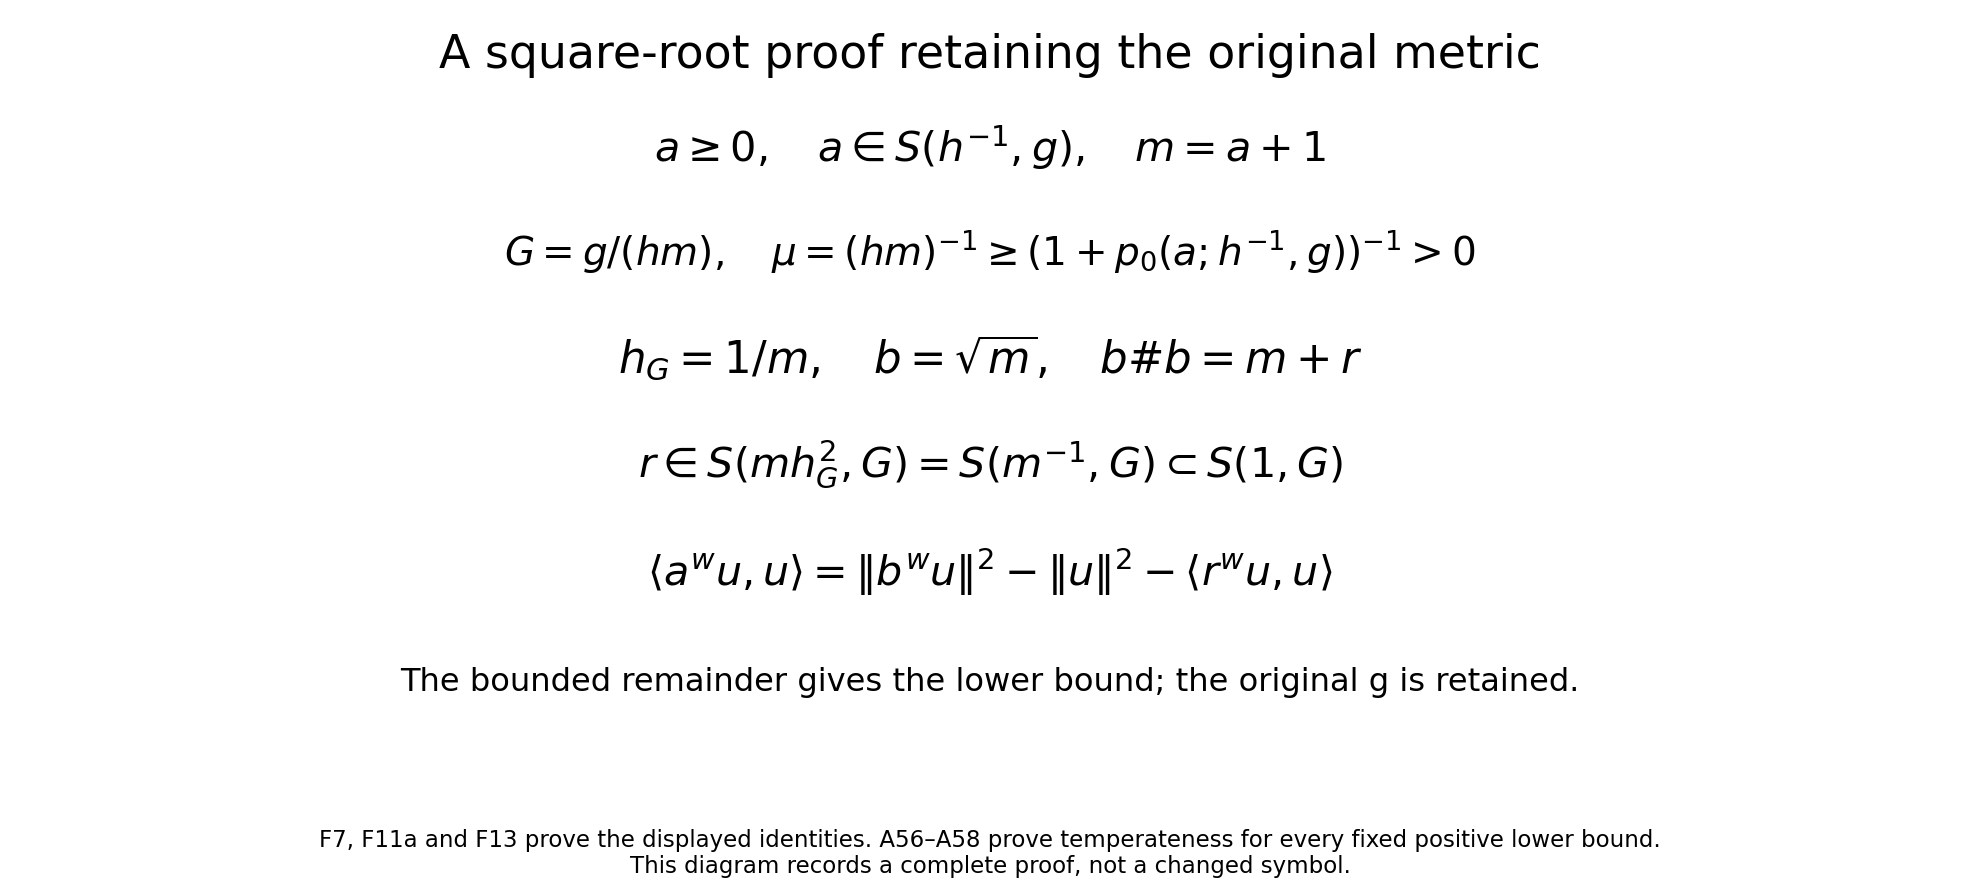
\includegraphics[keepaspectratio]{../figures/adapted-square-original-metric.png}}
\caption{The adapted square on the original metric}
\end{figure}

The diagram keeps the original \(g,h,a\) and every factor in (F7),
(F11a), (F13). Equations (A56)--(A58) prove the conformal comparison
used here. This calculation uses the original conformal factor without a
metric replacement.

\ReaderArmAliases{\ReaderOriginalAnchorStart{AN03-SFP-010}\ReaderOriginalAnchorEnd\begingroup\expandafter\def\csname @currentHref\endcsname{AN03-SFP-010}\label{AN03-SFP-010}\endgroup\ReaderOriginalAnchorStart{an03-sfp-010-why-the-inverse-square-is-the-last-uniform-power}\ReaderOriginalAnchorEnd\begingroup\expandafter\def\csname @currentHref\endcsname{an03-sfp-010-why-the-inverse-square-is-the-last-uniform-power}\label{an03-sfp-010-why-the-inverse-square-is-the-last-uniform-power}\endgroup\ReaderOriginalAnchorStart{10-why-the-inverse-square-is-the-last-uniform-power}\ReaderOriginalAnchorEnd\begingroup\expandafter\def\csname @currentHref\endcsname{10-why-the-inverse-square-is-the-last-uniform-power}\label{10-why-the-inverse-square-is-the-last-uniform-power}\endgroup\ReaderOriginalAnchorStart{why-the-inverse-square-is-the-last-uniform-power}\ReaderOriginalAnchorEnd}
\subsection{10. Why the inverse square is the last uniform
power}\label{why-the-inverse-square-is-the-last-uniform-power}

In one spatial dimension let \(b(x,\xi)=x\xi\) and \(p=b^2\). The exact
polynomial Weyl product is \[
b\#b=b^2+\frac14,
\qquad \langle p^wu,u\rangle=\|b^wu\|^2-\frac14\|u\|^2.
\tag{F42}
\] For a direct check, \(b^w=-i(x\partial_x+1/2)\), whereas
\((x^2\xi^2)^w=-x^2\partial_x^2-2x\partial_x-1/2\). Squaring the first
expression gives the second plus \(1/4\).

Choose a nonzero real \(\eta\in C_c^\infty((0,1))\) and, for \(L>1\),
set \[
u_L(x)=x^{-1/2}\eta((\log x)/L)\quad(x>0),
\qquad u_L(x)=0\quad(x\leq0).
\tag{F43}
\] Each function is smooth with compact support away from zero.
Substituting \(t=\log x\) gives \[
\|u_L\|^2=L\|\eta\|^2,
\qquad \|b^wu_L\|^2=L^{-1}\|\eta'\|^2.
\tag{F44}
\] For one fixed sufficiently large \(L\), (F42) is strictly negative.
This is an independently chosen logarithmic test family; it uses no
spectral assertion about the dilation generator.

Let \(\theta\geq0\) be smooth, compactly supported on phase space, and
equal to one near zero. Put \(p_0(X)=\theta(X)p(X)\geq0\). Then \[
\lambda^{-2}p_0(\sqrt\lambda X)
=\theta(\sqrt\lambda X)p(X)\longrightarrow p(X)
\quad\text{in }\mathcal S'(\mathbb R^2),
\tag{F45}
\] as \(\lambda\downarrow0\): the convergence is pointwise and bounded
by a fixed quartic polynomial, so dominated convergence applies against
each Schwartz function. Pairing with the Wigner function of the fixed
\(u_L\) yields \[
\lambda^{-2}\langle p_0(\sqrt\lambda\,\cdot)^wu_L,u_L\rangle
\longrightarrow\langle p^wu_L,u_L\rangle<0.
\tag{F46}
\] Fix \(s>2\), and define
\(a_\lambda(X)=\lambda^{-s}p_0(\sqrt\lambda X)\), with constant metric
\(g_\lambda=\lambda e\). Then \(h_{g_\lambda}=\lambda\), and \[
p_k(a_\lambda;\lambda^{-s},g_\lambda)
=\sup_X|p_0^{(k)}(X)|.
\tag{F47}
\] Thus every relevant symbol seminorm is uniform, but the quadratic
form in (F46), multiplied by \(\lambda^{2-s}\), tends to minus infinity.
A fixed positive rescaling of \(p_0\) can make any prescribed finite
list of these seminorms at most one; it does not change the divergence.
No uniform theorem of the constant-metric form (F31) can replace
\(\lambda^{-2}\) by \(\lambda^{-s}\).

One can also put this obstruction into a single variable metric and a
single symbol. This avoids interpreting a family of metrics as though it
were one fixed operator. Still in one phase plane, take \[
g_X=\langle X\rangle^{-1}e,\quad h(X)=\langle X\rangle^{-1},
\quad R_j=2^{2^{j+j_0}},\quad X_j=(R_j,0),
\quad A(X)=\sum_{j\geq1}R_j^s p_0((X-X_j)/\sqrt{R_j}).
\tag{F48}
\] Choose the fixed integer \(j_0\) sufficiently large. The summands
then have disjoint supports, of radius at most a fixed multiple of
\(\sqrt{R_j}\), so the sum is locally finite and nonnegative. On each
support \(\langle X\rangle\) is comparable to \(R_j\); differentiating
the summand proves \(A\in S(h^{-s},g)\). Slow variation of this metric
follows from \(|\langle X\rangle-\langle Y\rangle|\leq|X-Y|\), and
(F29), with \(H=\langle X\rangle^{-1}\), proves symplectic
temperateness. Its uncertainty inequality holds.

Let \(v_j\) be the unitary phase translation of the one fixed test
function \(u_L\) to \(X_j\). The contribution of the \(j\)-th summand to
its quadratic form is at most \(-cR_j^{s-2}\) for large \(j\), by (F46).
Every other contribution is negligible in absolute value. Here is a
quantitative justification. The Wigner function of \(u_L\) is Schwartz,
and the kernel formula (F1) pairs it with the symbol, up to the fixed
factor \((2\pi)^{-1}\). For any integer \(M\), the absolute contribution
of the \(k\)-th summand with \(k\ne j\) is at most \[
C_M R_k^{s+1}(1+|X_k-X_j|)^{-M}.
\tag{F49}
\] The power \(R_k\) in the volume factor is the area of its phase-space
support. The chosen growth of the centers makes that support's radius
negligible relative to the distance between different centers. For
\(k<j\), the sum of (F49) is at most \(C_MR_j^{-M}R_{j-1}^{s+1}\); for
\(k>j\), it is at most \(C_M\sum_{k>j}R_k^{s+1-M}\). Taking \(M>s+3\)
makes both bounds tend to zero. The fixed \(L^2\) norm of \(v_j\)
therefore accompanies a quadratic form tending to minus infinity. Thus
the general theorem with \(h^{-s}\), \(s>2\), fails even for one
permissible metric and one nonnegative scalar symbol.

The example concerns scalar Weyl positivity and the uniform exponent. It
neither gives an operator-valued Fefferman--Phong theorem nor supplies
the separate matrix counterexamples needed to classify that setting.

\ReaderArmAliases{\ReaderOriginalAnchorStart{AN03-SFX-001}\ReaderOriginalAnchorEnd\begingroup\expandafter\def\csname @currentHref\endcsname{AN03-SFX-001}\label{AN03-SFX-001}\endgroup\ReaderOriginalAnchorStart{an03-sfx-001-examples-separating-the-assumptions}\ReaderOriginalAnchorEnd\begingroup\expandafter\def\csname @currentHref\endcsname{an03-sfx-001-examples-separating-the-assumptions}\label{an03-sfx-001-examples-separating-the-assumptions}\endgroup\ReaderOriginalAnchorStart{11-examples-separating-the-assumptions}\ReaderOriginalAnchorEnd\begingroup\expandafter\def\csname @currentHref\endcsname{11-examples-separating-the-assumptions}\label{11-examples-separating-the-assumptions}\endgroup\ReaderOriginalAnchorStart{examples-separating-the-assumptions}\ReaderOriginalAnchorEnd}
\subsection{11. Examples separating the
assumptions}\label{examples-separating-the-assumptions}

\textbf{Subtracting a constant from a positive square.} The operator
\((xD+D x)^2/4\) is nonnegative on Schwartz functions, and its Weyl
symbol is \(x^2\xi^2+1/4\). Subtracting \(1/4\) leaves the nonnegative
symbol \(x^2\xi^2\), but its operator has negative test forms by
(F42)--(F44). Positivity of a function and positivity of its
quantization are two different statements even for a polynomial.

\textbf{A singular zero set without a positive Hessian.} The function
\(f(s,y)=s^4+y^6\) has both value and Hessian zero at the origin. The
adaptive scale there is at its floor. The proof does not invoke an
implicit critical graph with a nonzero Hessian at that point. It uses an
ordinary bounded-symbol estimate on that scale, while nearby points with
a larger value or Hessian can use the splitting argument. This is why
the theorem includes arbitrarily degenerate zeros.

\textbf{A classical symbol at a nonclassical derivative scale.} Let
\(\rho=3/4\), \(\delta=1/4\), and let \(F\geq0\) be smooth on
\(\mathbb R\) with every derivative bounded. In one dimension, \[
a(x,\xi)=\langle\xi\rangle
 F(x\langle\xi\rangle^{1/4})\chi(x)
\tag{F50}
\] belongs to \(S_{3/4,1/4}^{1}\) if \(\chi\geq0\) is smooth with
compact support. To check the frequency derivatives, every derivative of
the composed argument produces a factor bounded on
\(\operatorname{supp}\chi\) by \(C\langle\xi\rangle^{-3/4}\); subsequent
derivatives improve this bound. An \(x\) derivative costs at most
\(\langle\xi\rangle^{1/4}\). The product rule gives the asserted class.
Since \(1=2(\rho-\delta)\), (F40) applies. This example illustrates the
derivative accounting; the theorem is not restricted to such separated
symbols or to compact support in \(x\).

\ReaderArmAliases{\ReaderOriginalAnchorStart{AN03-SFQ-001}\ReaderOriginalAnchorEnd\begingroup\expandafter\def\csname @currentHref\endcsname{AN03-SFQ-001}\label{AN03-SFQ-001}\endgroup\ReaderOriginalAnchorStart{an03-sfq-001-problems-and-complete-solutions}\ReaderOriginalAnchorEnd\begingroup\expandafter\def\csname @currentHref\endcsname{an03-sfq-001-problems-and-complete-solutions}\label{an03-sfq-001-problems-and-complete-solutions}\endgroup\ReaderOriginalAnchorStart{12-problems-and-complete-solutions}\ReaderOriginalAnchorEnd\begingroup\expandafter\def\csname @currentHref\endcsname{12-problems-and-complete-solutions}\label{12-problems-and-complete-solutions}\endgroup\ReaderOriginalAnchorStart{problems-and-complete-solutions}\ReaderOriginalAnchorEnd}
\subsection{12. Problems and complete
solutions}\label{problems-and-complete-solutions}

\textbf{Problem 1.} For a constant metric
\(g=\alpha\,dx^2+\beta\,d\xi^2\) on one phase plane, compute its dual
and Planck parameter. Find a symplectic dilation making its two
coefficients equal.

\textbf{Solution.} Formula (F2) gives
\(g^\sigma=\beta^{-1}dx^2+\alpha^{-1}d\xi^2\), so \(h^2=\alpha\beta\).
Under \((x,\xi)=(cy,c^{-1}\eta)\), the coefficients become
\(\alpha c^2\) and \(\beta c^{-2}\). Taking \(c=(\beta/\alpha)^{1/4}\)
makes both equal to \(\sqrt{\alpha\beta}=h\). The map preserves
\(dx\wedge d\xi\); its unitary action on functions is the corresponding
normalized dilation. Thus arbitrary eccentricity does not enter the
constant-metric lower bound.

\textbf{Problem 2.} Why does a single square-root argument applied
naively to \(a+1\) at size \(h^{-2}\) fail to prove the second line of
(F5)?

\textbf{Solution.} For a general nonnegative symbol of that size, the
first-derivative positivity estimate is
\(|a'|\lesssim\sqrt{a}\,h^{-1}g^{1/2}\). The natural conformal metric
that makes \(a+1\) its own weight is then \(G=(a+1)^{-1}h^{-2}g\). Its
Planck parameter is \(h_G=(a+1)^{-1}h^{-1}\), which can exceed one near
a zero of \(a\). The Weyl square remainder also has weight
\((a+1)h_G^2=(a+1)^{-1}h^{-2}\), which need not be bounded. The scalar
splitting and dimensional reduction resolve precisely this failure; a
formal square root alone does not.

\textbf{Problem 3.} Verify the cancellation in (F23) and state the
remaining weight when \(a\) has weight \(h^{-2}\).

\textbf{Solution.} The Leibniz rule gives
\(\{\phi a,\phi\}=\phi\{a,\phi\}+a\{\phi,\phi\}=-\phi\{\phi,a\}\).
Scalar multiplication commutes, so it cancels \(\{\phi,a\}\phi\). The
first surviving terms contain two symplectic contractions. Their weight
is \(h^{-2}h^2=1\), both for the direct second correction and for the
composition of two first corrections. That is why the localization error
is bounded in \(L^2\).

\textbf{Problem 4.} Suppose \(a^{(k)}\) satisfies (F25) and \(H\) is
defined by (F26). Explain both inequalities \(\lambda\leq H\leq1\), and
compute the rescaled \(k\)-th derivative in (F27).

\textbf{Solution.} The maximum defining \(H^{-1}\) is at least one. Its
other two entries are at most \(\lambda^{-1}\), by the order-zero and
order-two bounds in (F25); since \(\lambda\leq1\), the maximum is at
most \(\lambda^{-1}\). Thus \(\lambda\leq H\leq1\). The chain rule gives
\(f_X^{(k)}=H^{2-k/2}a^{(k)}(X+H^{-1/2}z)\). For \(k\geq4\), its norm is
at most \((\lambda/H)^{(k-4)/2}\leq1\). The lower derivative bounds
instead use nonnegativity and the jet lemma; (F25) alone would give
negative powers of \(\lambda/H\) there.

\textbf{Problem 5.} For the logarithmic family (F43), prove the
negative-form condition and explain why one fixes \(L\) before letting
\(\lambda\) tend to zero.

\textbf{Solution.} Equations (F42) and (F44) give
\(\langle p^wu_L,u_L\rangle=L^{-1}\|\eta'\|^2-(L/4)\|\eta\|^2\),
negative when \(L^2>4\|\eta'\|^2/\|\eta\|^2\). Fix such an \(L\). Its
Wigner function is now one fixed Schwartz test function, so the
distributional convergence in (F45) gives (F46) directly. Letting the
test function change with \(\lambda\) would require a separate uniform
convergence estimate; none is needed for this counterexample.

\textbf{Problem 6.} A localized splitting has a profile \(v\)
independent of one phase direction but supported only on a transverse
ball. Describe a global extension preserving the direction independence
and nonnegativity, and explain why cutting off in all phase directions
at that step is unsuitable.

\textbf{Solution.} Project the compact support of \(\chi\) onto the
orthogonal complement of the constant direction. This projection lies
strictly inside the transverse domain on which \(v\) is defined. Choose
a nonnegative transverse cutoff equal to one near this projection and
supported inside that domain. Multiply \(v\) by it and extend by zero in
the transverse variables; leave the constant direction unrestricted. The
extension is smooth, nonnegative and independent of that direction, and
satisfies \(\chi^2\widetilde v=\chi^2v\). The later factor \(\chi\)
supplies the remaining localization in (F33). A cutoff varying in the
missing direction would destroy the parameter decomposition used in
dimension induction.

\ReaderArmAliases{\ReaderOriginalAnchorStart{AN03-SFP-SOURCE-001}\ReaderOriginalAnchorEnd\begingroup\expandafter\def\csname @currentHref\endcsname{AN03-SFP-SOURCE-001}\label{AN03-SFP-SOURCE-001}\endgroup\ReaderOriginalAnchorStart{exact-source-comparisons-and-visible-corrections}\ReaderOriginalAnchorEnd}
\subsection{13. Exact source comparisons and visible
corrections}\label{exact-source-comparisons-and-visible-corrections}

The following is a separate editorial comparison, keeping the preceding
scalar theorem and proof intact. It compares Wen Deng, \emph{Structure
constants of the Weyl calculus}, arXiv:1109.4793v1, with the original
course formulas (F1)--(F5) and (F42). The source's own wording and valid
theorem remain identifiable. The two source-text corrections below are
not errors in the course's independent scalar proof. The original author
files have not been edited. There is no novelty claim.

The original source uses a measurable positive quadratic metric, the
symplectic form \(\sigma=\sum_jd\xi_j\wedge dx_j\), a continuous
confined-symbol partition and imported Wiener and biconfinement
theorems. The comparisons below apply on that common measurable-metric
scope. They do not use the source to certify a larger nonmeasurable
scope or to supply the missing proofs in its cited books.

\subsubsection{13.1. Every Fourier and metric factor in the
comparison}\label{every-fourier-and-metric-factor-in-the-comparison}

Keep the original course symbol \(a(x,\xi)\), its original metric \(g\),
original symplectic form and Lebesgue measure. Put \(c=2\pi\) and
introduce only the comparison map \[
 L(x,\eta)=(x,c\eta),\qquad \det L=c^n,
 \qquad a_D=a\circ L.
 \tag{SD1}
\] For a Schwartz symbol and test function, substitution \(\xi=c\eta\)
in the absolutely convergent source quantization gives \[
 \begin{aligned}
 (a_D)^w_Du(x)
 &=\iint e^{ic(x-y)\cdot\eta}
      a((x+y)/2,c\eta)u(y)\,dy\,d\eta\\
 &=c^{-n}\iint e^{i(x-y)\cdot\xi}
      a((x+y)/2,\xi)u(y)\,dy\,d\xi
 =a^wu(x).
 \end{aligned}
 \tag{SD2}
\] For a tempered symbol the same identity is an equality of
distributional kernels. Here is the exact extension, rather than an
ordinary integral assertion: the partial Fourier transform is a
continuous bijection of the Schwartz space and its distribution dual,
and the coordinate change \((x,y)\mapsto((x+y)/2,x-y)\) is invertible.
They define both kernel maps continuously on tempered symbols. The
distribution pullback under \(L\) is
\(\langle a_D,\varphi\rangle=c^{-n}\langle a,\varphi\circ L^{-1}\rangle\).
Applying these continuous maps to this identity gives precisely (SD2),
including its \(c^{-n}\). Equivalently one may test against the Schwartz
Wigner function of two Schwartz functions; the same substitution has the
same determinant. The complete Fourier, linear-substitution and
distribution maps are already proved in the course prerequisites cited
before (F2).

For all vectors \(T,S\), \(\sigma(LT,LS)=c\sigma(T,S)\). Write
\(\widetilde g=L^*g\), meaning \(\widetilde g_Y(T)=g_{LY}(LT)\). Its
original symplectic dual is \[
 \begin{aligned}
 \widetilde g_Y^\sigma(T)
 &=\sup_{S\ne0}\frac{\sigma(T,S)^2}{g_{LY}(LS)}
 =c^{-2}g_{LY}^\sigma(LT),\\
 \widehat g&=c^{-1}L^*g,
 \qquad \widehat g_Y^\sigma=c^{-1}L^*(g^\sigma)_Y.
 \end{aligned}
 \tag{SD3}
\] The second line uses the exact rule \((bq)^\sigma=b^{-1}q^\sigma\)
for \(b>0\), proved directly from the quotient defining the dual. Thus
\(\widehat g\le\widehat g^\sigma\) is equivalent to the original
\(g\le g^\sigma\). The map has not replaced the original metric in the
course calculation.

The original course quantity is
\(h(X)^2=\sup_{T\ne0}g_X(T)/g_X^\sigma(T)\). The source quantity is the
reciprocal ratio, not the same quantity: \[
 h_{\widehat g}(Y)=h(LY),\qquad
 \lambda_{\widehat g}(Y)
 =\inf_{T\ne0}\left(\frac{\widehat g_Y^\sigma(T)}{\widehat g_Y(T)}\right)^{1/2}
 =h(LY)^{-1}.
 \tag{SD4}
\] The positive ratios attain finite positive extrema on a Euclidean
unit sphere; reciprocating therefore changes their supremum into the
reciprocal infimum. This also proves the identity at every base point
without an exceptional zero or infinite value.

For the exact order-\(k\) directional seminorm, with the original weight
\(h^{-2}\), the full comparison is \[
 p_k(a_D;(h\circ L)^{-2},\widehat g)
 =c^{k/2}p_k(a;h^{-2},g).
 \tag{SD5}
\] A \(\widehat g\)-unit vector maps to a vector of original
\(g\)-length \(\sqrt c\); each of the \(k\) arguments contributes that
factor. Conversely every such original vector is obtained by the inverse
map. The weight has unchanged value at the corresponding point. For the
source maximum through order \(l\), the exact expression is
\(\max_{0\le k\le l}c^{k/2}p_k(a;h^{-2},g)\), bounded by
\(c^{l/2}\max_{0\le k\le l}p_k(a;h^{-2},g)\). Do not substitute that
upper bound for the exact maximum.

Slow variation retains its full radius: if \(g\) has comparison constant
\(C_0\) for original squared distance at most \(C_0^{-1}\), then the
same comparison applies when \(\widehat g_Y(Y-Z)\le(cC_0)^{-1}\). In the
original distance \(g_{LY}^\sigma(L(Y-Z))=c\widehat g_Y^\sigma(Y-Z)\). A
one-base temperateness power \(N\) consequently retains the factor
\(c^N\) as an upper bound when expressed with
\(1+\widehat g_Y^\sigma(Y-Z)\). Section2 below gives the exact
comparison with the source's harmonic-mean distance. Together
(SD2)--(SD5) identify the lower-bound conclusions on their common scope
with finite structural and symbol constants retained.

The polynomial correction is equally explicit. With the original
\(D=-i\partial_x\), let \(K=(xD+Dx)/2\). Original (F42) gives
\((x^2\xi^2)^w=K^2-1/4\). The source operator for the unscaled
coordinate symbol \(x\eta\) is \(K/c\), and \[
 (x^2\eta^2)^w_D=c^{-2}(K^2-1/4)
 =(K/c)^2-\frac{1}{4c^2}
 =(K/c)^2-\frac{1}{16\pi^2}.
 \tag{SD6}
\] Here \((x^2\xi^2)\circ L=c^2x^2\eta^2\) and linearity supply the
factor \(c^{-2}\); no square constant has been deleted or identified
with a differently scaled symbol.

\subsubsection{13.2. The exact two-way temperateness
map}\label{the-exact-two-way-temperateness-map}

Let \(Q_X=g_X^\sigma\). Suppose the original (F3) holds in its actual
orientation: \[
 g_Y\le Cg_X(1+Q_Y(X-Y))^N,
 \qquad C\ge1,\quad N\ge0.
 \tag{SD7}
\] For \(d=X-Y\) minimize \(Q_X(u)+Q_Y(v)\) under \(u+v=d\). In the
original symmetric positive matrices the unique critical point and
minimum are \[
 \begin{aligned}
 u&=(Q_X+Q_Y)^{-1}Q_Yd,\qquad v=d-u,\\
 A+B&:=Q_X(u)+Q_Y(v)
 =d^T(Q_X^{-1}+Q_Y^{-1})^{-1}d
 =\tfrac12(Q_X\wedge Q_Y)(d),\\
 Q_X\wedge Q_Y&=2(Q_X^{-1}+Q_Y^{-1})^{-1}.
 \end{aligned}
 \tag{SD8}
\] To prove the minimum, expand \(u^TQ_Xu+(d-u)^TQ_Y(d-u)\), complete
the square with matrix \(Q_X+Q_Y\), and retain the remaining matrix
\(Q_Y-Q_Y(Q_X+Q_Y)^{-1}Q_Y\). It equals \(Q_Y(Q_X+Q_Y)^{-1}Q_X\). Its
inverse is \(Q_X^{-1}(Q_X+Q_Y)Q_Y^{-1}=Q_Y^{-1}+Q_X^{-1}\); this proves
(SD8) without commuting the original matrices.

Put \(Z=X-u=Y+v\). The orientation of (SD7) gives
\(g_X\le Cg_Z(1+A)^N\). Duality gives \(Q_Z\le C Q_X(1+A)^N\). A second
application gives \[
 g_Z\le Cg_X(1+Q_Z(u))^N
 \le Cg_X[1+CA(1+A)^N]^N.
\] Also \(g_Y\le Cg_Z(1+B)^N\). Since
\(1+CA(1+A)^N\le(1+C)(1+A)^{N+1}\), multiplication gives the complete
source-distance bound \[
 \begin{aligned}
 g_Y
 &\le C^2(1+C)^N g_X(1+A+B)^{N^2+2N}\\
 &\le C^2(1+C)^N g_X
       [1+(Q_X\wedge Q_Y)(X-Y)]^{N^2+2N}.
 \end{aligned}
 \tag{SD9}
\] The source orientation with \(g_X\) on the left follows by
interchanging \(X,Y\); the mean is symmetric. Conversely choose
\(u=d,v=0\) in the minimum: \((Q_X\wedge Q_Y)(d)\le2Q_X(d)\), and choose
\(u=0,v=d\) to obtain the separate bound by \(2Q_Y(d)\). Therefore a
harmonic-mean temperateness bound with constant \(C_D\) and power
\(N_D\) implies (SD7) with \(C_D2^{N_D}\) and \(N_D\). This proves both
maps, including the case \(N=0\).

\subsubsection{13.3. The corrected quadratic-cutoff derivatives and
their full
receiver}\label{the-corrected-quadratic-cutoff-derivatives-and-their-full-receiver}

In source Section2, original TeX line223 misses a factor2. Fix the
original base \(Y\), positive quadratic form \(g_Y\), its associated
inner product, original radius \(r>0\), and the actual smooth
nonincreasing cutoff \(\chi_0\), with \(\chi_0=1\) for arguments at most
\(1/2\), \(\chi_0=0\) for arguments at least1, and \(0\le\chi_0\le1\).
Write \(z=X-Y\), \(q_Y(X)=r^{-2}g_Y(z)\), and
\(\omega_Y(X)=\chi_0(q_Y(X))\). The exact first derivative is \[
 D\omega_Y(X)[T]
 =2r^{-2}\chi_0'(r^{-2}g_Y(X-Y))\langle X-Y,T\rangle_Y.
 \tag{SD10}
\] Indeed \(g_Y(z+tT)=g_Y(z)+2t\langle z,T\rangle_Y+t^2g_Y(T)\). This is
fixed by the original quadratic form; changing the meaning of its
associated inner product would change the original data.

For every \(k\ge1\), the entire repeated-direction formula is \[
 D^k\omega_Y(X)[T^k]
 =\sum_{p=\lceil k/2\rceil}^{k}
 \frac{k!\,2^{2p-k}}{(2p-k)!(k-p)!}
 \chi_0^{(p)}(r^{-2}g_Y(z))r^{-2p}
 \langle z,T\rangle_Y^{2p-k}g_Y(T)^{k-p}.
 \tag{SD11}
\] Taylor-expand the original \(\chi_0\) through order \(k\) in the
increment \(r^{-2}(2t\langle z,T\rangle_Y+t^2g_Y(T))\). The order-\(p\)
power contributes to \(t^k\) only by choosing \(2p-k\) linear factors
and \(k-p\) quadratic factors. Multiplying its coefficient by \(k!\),
including the Taylor \(1/p!\), gives exactly (SD11). The Taylor
remainder is \(o(t^k)\), so this coefficient calculation proves the
derivative even where some factors vanish. At order zero the expression
is just \(\chi_0(q_Y)\).

Every mixed direction is retained as well. If \(\Pi_k^{1,2}\) denotes
the set of partitions of \(\{1,\ldots,k\}\) whose blocks have size1 or2,
then \[
 \begin{aligned}
 D^k\omega_Y(X)[T_1,\ldots,T_k]
 &=\sum_{\pi\in\Pi_k^{1,2}}\chi_0^{(|\pi|)}(q_Y(X))
       \prod_{B\in\pi}D^{|B|}q_Y(X)[T_i:i\in B],\\
 Dq_Y[T_i]&=2r^{-2}\langle z,T_i\rangle_Y,
 \qquad D^2q_Y[T_i,T_j]=2r^{-2}\langle T_i,T_j\rangle_Y.
 \end{aligned}
 \tag{SD12}
\] All derivatives of \(q_Y\) of order at least3 vanish. Repeated
differentiation of the product adds the new index either as a singleton
differentiating \(\chi_0\), or to a singleton block differentiating
\(Dq_Y\). These choices generate each new partition exactly once;
adjoining it to a double block gives zero. This proves (SD12) by
induction and proves the full mixed formula without omitting
multiplicities.

For \(k\ge1\) define the actual finite coefficient sum \[
 C_k(\chi_0)=\sum_{p=\lceil k/2\rceil}^{k}
 \frac{k!\,2^{2p-k}}{(2p-k)!(k-p)!}\|\chi_0^{(p)}\|_\infty.
 \tag{SD13}
\] On the support of a nonzero term, \(g_Y(z)\le r^2\). Cauchy--Schwarz
gives \(|\langle z,T\rangle_Y|\le r g_Y(T)^{1/2}\). Thus every original
power in (SD11) gives \[
 |D^k\omega_Y(X)[T^k]|
 \le C_k(\chi_0)r^{-k}g_Y(T)^{k/2}
 \le C_k(\chi_0)r^{-k}C_0^{k/2}g_X(T)^{k/2},
 \quad r^2\le C_0^{-1}.
 \tag{SD14}
\] The last comparison applies slow variation at base \(Y\), on the very
support just identified. In (SD12) each singleton contributes at most
\(2r^{-1}g_Y(T_i)^{1/2}\) and each double block at most
\(2r^{-2}g_Y(T_i)^{1/2}g_Y(T_j)^{1/2}\). The exact mixed bound is the
sum over \(\pi\), with coefficient
\(2^{|\pi|}\|\chi_0^{(|\pi|)}\|_\infty r^{-k}C_0^{k/2}\). Therefore the
source's estimates with unspecified finite constants keep their stated
order and support after the equality is corrected; the omitted2 is
restored in the constants explicitly.

The complete continuous-partition receiver keeps its original measure:
\[
 \omega(X,r)=\int_{\mathbb R^{2n}}\omega_Y(X)|g_Y|^{1/2}\,dY,
 \qquad \varphi_Y(X)=\omega_Y(X)/\omega(X,r).
 \tag{SD15}
\] Its lower bound is
\(\omega(X,r)\ge C_0^{-2n}r^{2n}\int\chi_0(|Z|^2)\,dZ>0\). To prove it,
where the comparison integrand is nonzero,
\(g_X(X-Y)\le r^2/C_0\le C_0^{-1}\), so \(g_Y(X-Y)\le C_0g_X(X-Y)\),
\(|g_Y|^{1/2}\ge C_0^{-n}|g_X|^{1/2}\), and monotonicity of \(\chi_0\)
applies. Substitution \(Z=C_0^{1/2}r^{-1}g_X^{1/2}(Y-X)\) has the full
Jacobian \(r^{2n}C_0^{-n}|g_X|^{-1/2}\), proving that bound. The
integral is positive since \(\chi_0=1\) on the ball \(|Z|^2\le1/2\).

On the original support, \(g_X(X-Y)\le C_0r^2\) and
\(|g_Y|^{1/2}\le C_0^n|g_X|^{1/2}\). Hence \[
 \begin{aligned}
 \omega(X,r)&\le C_0^{2n}r^{2n}|B_{2n}|,\\
 |D^k\omega(X,r)[T^k]|
 &\le C_k(\chi_0)C_0^{2n+k/2}r^{2n-k}|B_{2n}|g_X(T)^{k/2}.
 \end{aligned}
 \tag{SD16}
\] Here \(|B_{2n}|\) is the actual Euclidean unit-ball volume; it has
not been absorbed into another object. Differentiation under the
integral is justified even for the source's measurable metric. Fix
\(X_0\), take \(g_{X_0}(X-X_0)\le\varepsilon^2\le C_0^{-1}\), and
consider a nonzero cutoff derivative. Two slow comparisons give \(g_Y\)
comparable with \(g_{X_0}\) by \(C_0^2\), and
\(g_{X_0}(Y-X_0)\le2C_0^2r^2+2\varepsilon^2\). Thus the integration
support lies in one finite ellipsoid, the determinant density is at most
\(C_0^{2n}|g_{X_0}|^{1/2}\), and (SD12) gives a fixed integrable bound
for every prescribed derivative on that neighborhood. For fixed \(Y\)
the integrand is smooth in \(X\); dominated convergence and the integral
form of the difference quotient prove each derivative and its
continuity. No differentiability of \(Y\mapsto g_Y\) was used.

The positive lower bound permits the full reciprocal chain formula \[
 D^k(\omega^{-1})[T_1,\ldots,T_k]
 =\sum_{\pi\in\Pi_k}(-1)^{|\pi|}|\pi|!\,
 \omega^{-1-|\pi|}\prod_{B\in\pi}D^{|B|}\omega[T_i:i\in B],
 \tag{SD17}
\] where \(\Pi_k\) contains all set partitions. Differentiating
\(t^{-1}\) gives \((-1)^p p!t^{-p-1}\); the same partition induction
proves this formula. All its bounds are finite by (SD16) and the lower
bound. The full product rule for \(\omega_Y\omega^{-1}\) therefore gives
the original smooth partition bounds. Finally
\(\int\varphi_Y(X)|g_Y|^{1/2}dY=\omega(X,r)/\omega(X,r)=1\), with its
original support and measure unchanged. This supplies the entire
receiver of the corrected derivative, rather than only a first-order
observation.

\subsubsection{13.4. The literal Wiener-domain defect and a proved
ambient
repair}\label{the-literal-wiener-domain-defect-and-a-proved-ambient-repair}

Source lines541--543 first restrict \(a\) to Schwartz functions and then
assert inclusion of all bounded smooth symbols with bounded derivatives.
The original constant \(a=1\) disproves that literal inclusion: it has
every required bounded derivative, but \(\sup_X|X_1a(X)|=\infty\), so it
is not Schwartz. It does not contradict the intended localized Fourier
condition.

Keep the original dimension \(d=2n\), original compact smooth lattice
cutoff \(\chi_0\), original locally finite partition
\(\sum_{j\in\mathbb Z^d}\chi_0(X-j)=1\), and original Fourier convention
\(\mathcal F_Df(\Xi)=\int e^{-2\pi iX\cdot\Xi}f(X)\,dX\). For a tempered
distribution introduce the separate ambient class \[
 \begin{aligned}
 \widetilde{\mathcal A}
 &=\{a\in\mathcal S'(\mathbb R^d):\omega_a\in L^1(\mathbb R^d)\},\\
 \omega_a(\Xi)&=\sup_{j\in\mathbb Z^d}|\mathcal F_D(\chi_j a)(\Xi)|,
 \quad \chi_j(X)=\chi_0(X-j),
 \quad \|a\|_{\widetilde{\mathcal A}}=\int\omega_a(\Xi)\,d\Xi.
 \end{aligned}
 \tag{SD18}
\] Each compactly supported distribution has a smooth Fourier transform
of polynomial growth: differentiate its action on the smooth exponential
multiplied by a fixed compact test cutoff equal to one on its support.
The distribution's finite-order bound on that compact set proves the
asserted polynomial estimate for every derivative. Thus the countable
supremum in (SD18) is measurable and the definition is meaningful. This
is explicitly an editorial ambient-domain repair, not a silent
alteration of the source's declaration.

For \(a=1\), translation gives \[
 \mathcal F_D(\chi_j)(\Xi)=e^{-2\pi ij\cdot\Xi}\mathcal F_D\chi_0(\Xi),
 \qquad \omega_1=|\mathcal F_D\chi_0|.
 \tag{SD19}
\] To prove its integrability and the full finite-derivative inclusion,
let \(a\in C^{d+1}\) have all coordinate derivatives through that order
bounded. Write \[
 \begin{aligned}
 M_0&=\|\chi_0\|_1\|a\|_\infty,\\
 M_{d+1}&=\max_{1\le i\le d}\sum_{b=0}^{d+1}
 \binom{d+1}{b}\|\partial_i^b\chi_0\|_1
                       \|\partial_i^{d+1-b}a\|_\infty.
 \end{aligned}
 \tag{SD20}
\] For \(|\Xi|\le1\), the transform has absolute value at most \(M_0\),
uniformly in \(j\). For \(|\Xi|>1\), choose \(i\) with
\(|\Xi_i|\ge|\Xi|/\sqrt d\). The full product derivative and integration
by parts give \[
 (2\pi i\Xi_i)^{d+1}\mathcal F_D(\chi_j a)
 =\mathcal F_D\left(\sum_{b=0}^{d+1}\binom{d+1}{b}
                   (\partial_i^b\chi_j)(\partial_i^{d+1-b}a)\right),
 \tag{SD21}
\] and hence
\(\omega_a(\Xi)\le(2\pi)^{-d-1}d^{(d+1)/2}M_{d+1}|\Xi|^{-d-1}\). Every
derivative term and its multiplicity has been retained. The actual polar
measure gives \[
 \|a\|_{\widetilde{\mathcal A}}
 \le |B_d|M_0+(2\pi)^{-d-1}d^{(d+1)/2}
           |S^{d-1}|M_{d+1}\int_1^\infty r^{-2}\,dr
 =|B_d|M_0+(2\pi)^{-d-1}d^{(d+1)/2}|S^{d-1}|M_{d+1}.
 \tag{SD22}
\] In particular all \(S^0_{0,0}\) symbols lie in the repaired ambient
class, and taking \(a=1\) proves the finiteness in (SD19). The same
proof holds for bounded weak derivatives through order \(d+1\), using
the already proved weak product rule and distributional integration by
parts. It does not infer the imported fourth-derivative scalar
lower-bound theorem from Fourier integrability alone.

For completeness the ambient repair has the actual functional properties
needed to state its inclusion. Let \(K=\operatorname{supp}\chi_0\), let
\(J_K=\{m\in\mathbb Z^d:m\in K-K\}\), and put \(N_K=|J_K|<\infty\).
There are at most \(N_K\) nonzero partition terms at any point: if one
index \(j_0\) meets that point, every other index differs from \(j_0\)
by an element of \(J_K\). Fourier inversion in (SD18) makes each
\(\chi_j a\) a continuous bounded function, with norm at most
\(\|a\|_{\widetilde{\mathcal A}}\). Summing the locally finite partition
identifies \(a\) as a continuous bounded function and proves \[
 \|a\|_\infty\le N_K\|a\|_{\widetilde{\mathcal A}}.
 \tag{SD23}
\] If the latter quantity is zero every \(\chi_j a\) vanishes, so the
distribution \(a\) vanishes. Triangle inequality and homogeneity follow
from the countable supremum and the integral; the original quantity is a
norm.

For a Cauchy sequence \(a_l\) in this norm, (SD23) gives a uniform limit
\(a\in C_b\). Each \(\chi_j a_l\) converges uniformly on its fixed
compact support, so its Fourier transform converges pointwise to that of
\(\chi_j a\). At fixed \(l\), the supremum of their pointwise limits is
at most the lower limit of the suprema. Fatou's lemma gives
\(\|a_l-a\|_{\widetilde{\mathcal A}}\le\liminf_{m\to\infty}\|a_l-a_m\|_{\widetilde{\mathcal A}}\).
It follows that \(a\) belongs to the class and that \(a_l\to a\) in its
original norm. Thus this repaired ambient space is complete.

For \(a,b\) in it the product is their actual continuous-function
product. In the localized identity
\(\chi_j ab=\sum_k(\chi_j a)(\chi_k b)\), only indices with
\(k-j\in J_K\) occur. Fourier transform of each product is convolution
with no multiplier under \(\mathcal F_D\). Each convolution is bounded
by \(\omega_a*\omega_b\); the complete finite sum therefore gives \[
 \omega_{ab}\le N_K(\omega_a*\omega_b),\qquad
 \|ab\|_{\widetilde{\mathcal A}}
 \le N_K\|a\|_{\widetilde{\mathcal A}}\|b\|_{\widetilde{\mathcal A}}.
 \tag{SD24}
\] Tonelli justifies the convolution integral and retains its full
factor \(N_K\). The original norm has not been rescaled to suppress that
factor. These proofs establish bounded continuous representatives,
completeness and continuous multiplication for the explicit ambient
repair. The source's separate imported Wiener-based sharp
fourth-derivative theorem and its imported biconfinement bounds remain
distinct literature dependencies.

\subsubsection{13.5. Precise receiving and historical
scope}\label{precise-receiving-and-historical-scope}

The accompanying diagram is an exact two-dimensional sample of Section3.
Its original matrix is
\(G=\begin{pmatrix}1/2&1/8\\1/8&1/4\end{pmatrix}\), radius \(r=1\),
displacement \(z=(1,1/2)\), and direction \(T=(4/5,-2/5)\). The positive
first pivot and determinant \(7/64\) prove positivity. Direct
multiplication gives \(g^\sigma=(64/7)g\), so this constant metric also
satisfies uncertainty and slow variation with \(C_0=1\). The original
line has \(g(z+tT)=11/16+(7/10)t+(7/25)t^2\) and derivative
\(7/10+(14/25)t\). The displayed orange arrow is exactly \((9/20)T\),
not a unit-vector replacement.

For this sample only, the diagram chooses \(\chi_0(q)=1-\eta(2q-1)\),
where \(h(s)=e^{-1/s}\) for \(s>0\), zero otherwise, and
\(\eta(s)=h(s)/(h(s)+h(1-s))\). Every right derivative of \(h\) at zero
is the limit of an exponential times a polynomial in \(s^{-1}\), hence
vanishes, since each power times \(e^{-1/s}\) tends to zero. Thus \(h\)
is smooth and flat there. The denominator is everywhere positive, and
\(\eta'=[h'(s)h(1-s)+h(s)h'(1-s)]/[h(s)+h(1-s)]^2\ge0\). Consequently
this particular cutoff is smooth, nonincreasing, equal to1 for
\(q\le1/2\) and zero for \(q\ge1\). It is one admissible instance of the
original cutoff hypotheses; (SD10)--(SD17) still hold for every original
cutoff satisfying those hypotheses. The solid derivative curve uses the
complete (SD10), while the dashed source expression is exactly half that
value.

(SD1)--(SD9) prove the exact symbol, operator, metric,
reciprocal-parameter and distance maps relating original (F1)--(F5) and
(F42) to the cited source theorem. (SD10)--(SD17) restore the derivative
equality and propagate it through every cutoff order and the full
continuous-partition receiver. (SD18)--(SD24) disprove only the literal
Schwartz-domain inclusion and supply the explicit repaired ambient space
and the full finite-derivative inclusion, with all original Fourier and
lattice factors.

No original course scalar theorem is replaced. Its original discrete
cover, scalar splitting, dimensional induction, squared localization and
logarithmic test remain the current independent proof. The exact version
compared here is
\href{https://arxiv.org/abs/1109.4793v1}{Deng1109.4793v1,
submitted22September2011}; its complete TeX and included bibliography
were read. Its imported book theorems have not been reconstructed from
their original-author TeX here. The two corrections are visible source
notes, with their complete arguments above.

\begin{figure}
\centering
\pandocbounded{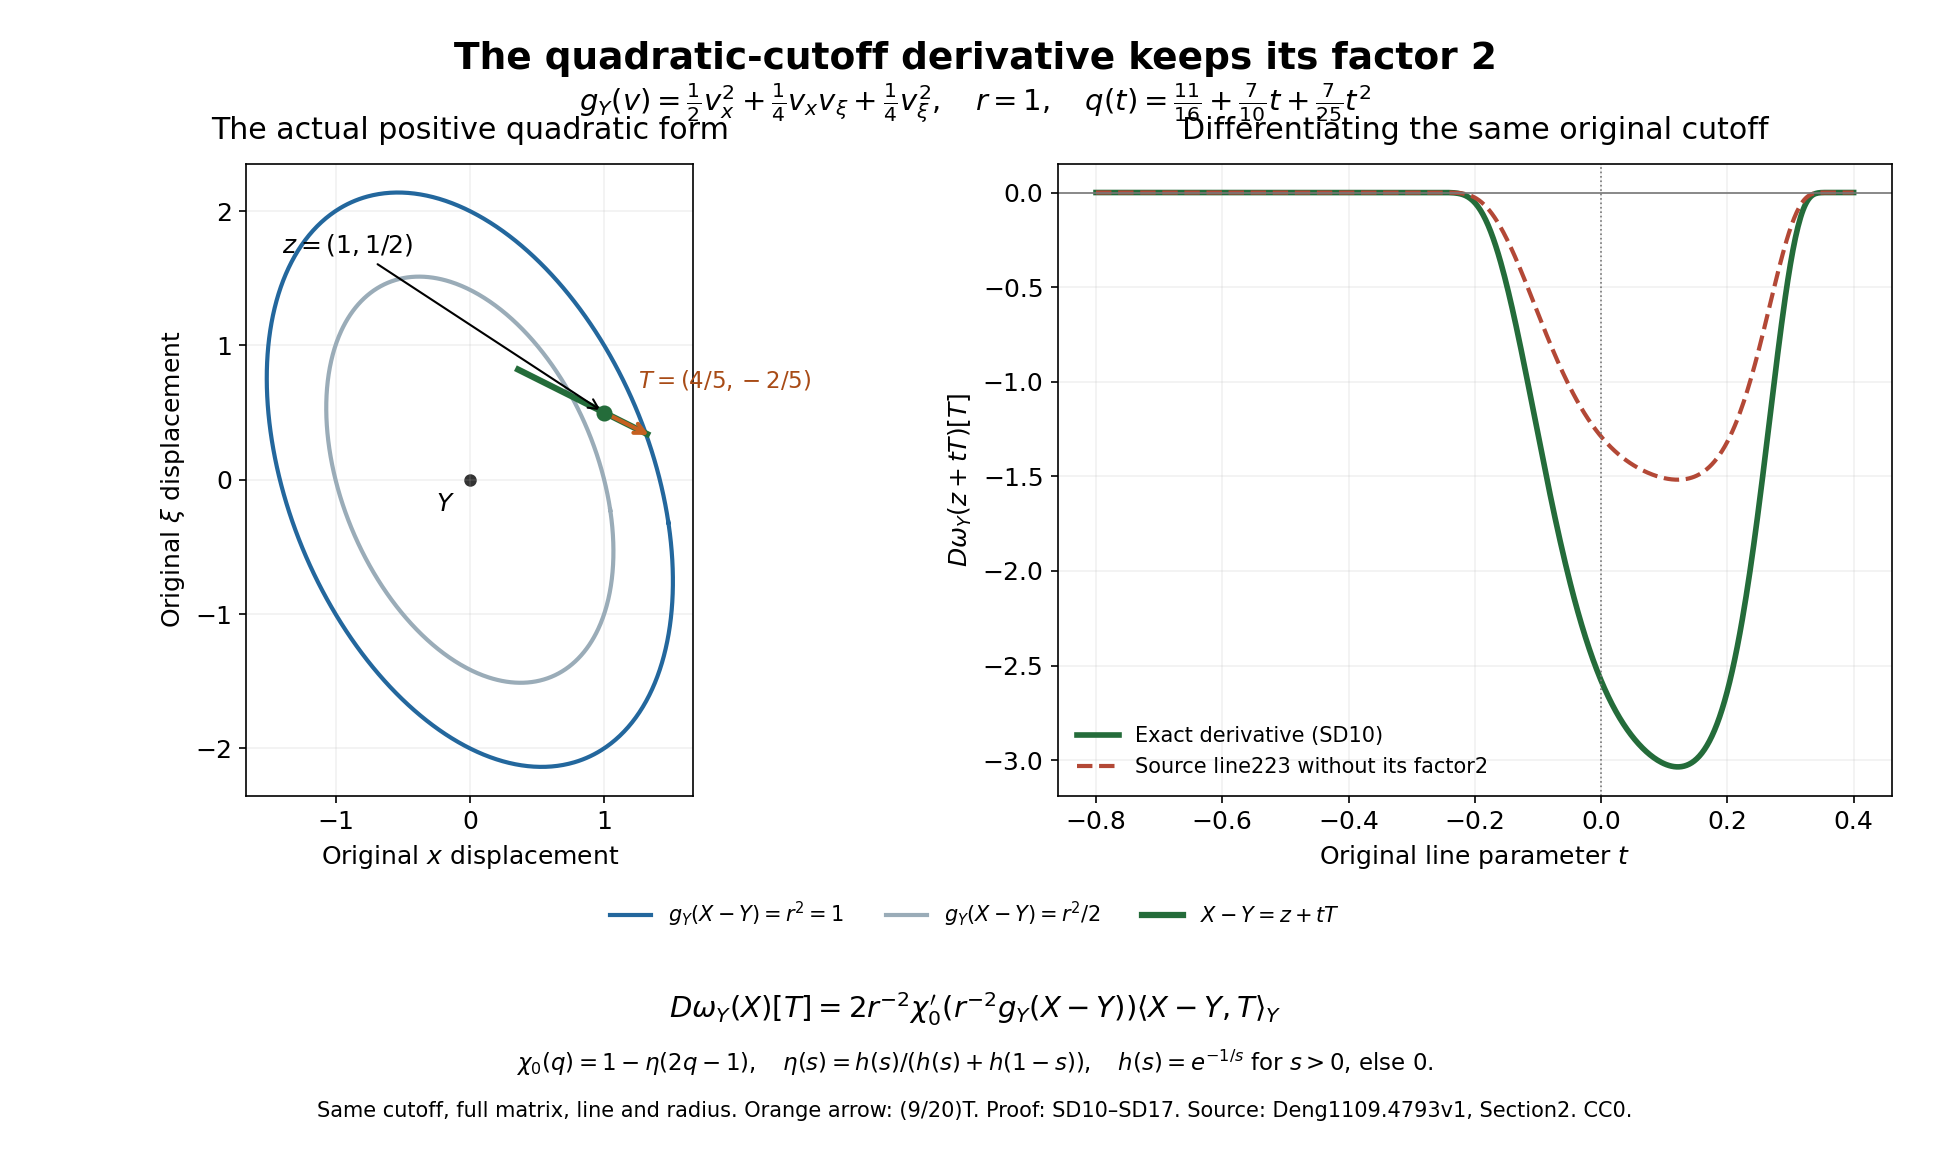
\includegraphics[keepaspectratio,alt={The original quadratic cutoff and its complete directional derivative}]{../figures/scalar-source-quadratic-cutoff.png}}
\caption{The original quadratic cutoff and its complete directional
derivative}
\end{figure}

The left panel retains the complete matrix, both original ellipsoids,
the displacement and direction. The right panel shows the exact
derivative and the source expression with its missing factor2; the
caption identifies the drawn arrow as (9/20)T. The exact sample and its
smooth cutoff are proved in Section13.5.

\ReaderArmAliases{\ReaderOriginalAnchorStart{reading-provenance-and-research-directions}\ReaderOriginalAnchorEnd\begingroup\expandafter\def\csname @currentHref\endcsname{reading-provenance-and-research-directions}\label{reading-provenance-and-research-directions}\endgroup\ReaderOriginalAnchorStart{references}\ReaderOriginalAnchorEnd}
\subsection{References}\label{references}

Wen Deng's \href{https://arxiv.org/abs/1109.4793v1}{\emph{Structure
constants of the Weyl calculus}, arXiv:1109.4793v1}, Theorem 4.1, states
the general-metric scalar bound on its declared measurable-metric scope,
with dependence on the metric's structural constants made explicit.
Section13 proves the exact operator and metric comparison and records
the two visible source corrections. Its proof uses a constant-metric
result formulated through fourth derivatives in a Wiener algebra,
followed by confined-symbol localization.

Nicolas Lerner's author-hosted
\href{https://webusers.imj-prg.fr/~nicolas.lerner/ch2booklerner.pdf}{\emph{Metrics
on the Phase Space}, chapter 2}, Theorems 2.5.5 and 2.5.10 and Remarks
2.5.13--14, discusses the general-metric bound and finer
fourth-derivative conditions. Its reciprocal Planck parameter and
\(2\pi\)-Fourier convention differ from (F1)--(F2). In particular
constants in a polynomial Weyl-square identity must be converted before
comparison.

\subsection{Further questions}\label{further-questions}

One direction for further work is an explicit, economical derivative
count in (F37) for a specified class of metric structural constants.
Another is to compare the sufficient pointwise condition \(a\geq0\) with
averaged conditions for a lower bound. Formula (F42) and the logarithmic
tests show that quantization can produce a bounded negative quadratic
form from a nonnegative scalar symbol. Sufficient averaged conditions
require a separate theorem; they do not follow by deleting nonnegativity
from the splitting lemma. A third direction is to identify exactly where
scalar multiplication and the scalar critical graph cease to work for
matrix symbols. The general Hilbert-valued sharp lower bound belongs to
its separate course unit, and an inverse-square improvement in that
setting cannot be inferred from this scalar proof.

\end{document}
